\newpage
\phantomsection
\chapter{Theoretical basis}\label{chap:theory}

There have been several theoretical and technical advances in optical coherence tomography (OCT) in response to the importance that it has gathered in the biomedical optics community. In this chapter, principle of operation, models for the OCT signal and advances of OCT are explained, including the different configurations that have been developed, starting from the initial approach based on low coherence interferometry in time domain detection that later advanced into spectral domain detection, and presenting advantages and disadvantages in practical features such as sensitivity, imaging speed, and most importantly here, phase stability that is discussed in detail. In the first part of this Chapter, Section~\ref{OCT}, the OCT experiment is analyzed from an interferometric perspective in regard to the coherence gating used for axial scan performed in OCT. In second part, Section~\ref{Model}, propagation of light in the sample arm is taken into account to establish a model for image formation in OCT, in regard to the confocal gating used for transverse scan. From this model derive the state-of-the-art techniques for computational aberration correction in OCT explained in Section~\ref{CAC}, where also phase stability requirement and approaches to achieved it are discussed.

\section{Optical coherence tomography}\label{OCT}

\textit{Tomography} techniques produce images by sectioning the sample using a penetrating wave~\cite{}. In medicine, tomography techniques radiate waves into the sample and measure the backscattered waves to produce cross-sectional images of the internal structure of tissues. For instance, ultrasound employs sound waves and measures the echo time delay and amplitude of the reflected waves~\cite{}, while light is used in optical coherence tomography~\cite{}. Measuring the echo time delay of light with micrometric resolution using direct electronic detection schemes as in ultrasound is challenging given that light is around six orders of magnitude faster than sound. Therefore, optical ranging measurements demand alternative approaches such as high-speed optical gating or low coherence interferometry that is the basis of OCT.

\subsection{Measuring the echo time delay of light}

Using backscattered light to see through biological tissue was proposed by Duguay~\cite{} in 1971 employing a high-speed optical Kerr shutter with a 10~pico-seconds pulsed laser to ``photograph light in flight'' while propagating through a cell of milk and water~\cite{}. In subsequent approaches, resolution was improved using nonlinear optical processes to detect the time delay of backscattered light with femto-second resolution, making possible to measure corneal thickness in a rabbit eye ex vivo with 15~$\mu m$ resolution~\cite{}. Drawbacks of these approaches are the use of intense pulsed lasers and that sensitivity is as low as $-$70~dB while current OCT systems achieve sensitivities of $-$100~dB, three order of magnitude greater.

\subsection{Low coherence interferometry}

Potential of low coherence interferometry to measure echo time delay of backscattered light with high resolution and sensitivity was devised in the 80s decade, starting with optical fibers and waveguide devices~\cite{} and later with biological samples after the first demonstration by Fercher et al. in 1986~\cite{} measuring the axial eye length. Interferometry techniques measures the correlation between optical fields by interfering light that is backscattered by the sample with light that has traveled through a reference path. In a interferometer, light emitted by the source is splitted into two arms, one is reflected by a reference mirror and the other is reflected by the sample, and then both are recombined to produce interference in a detection plane. Interference only occurs when the optical path length (OPL) difference between the two light beams is within the \textit{coherence length} of the light source $l_c$. This is the optical distance that different waves from the same light source can mismatch and yet maintain a \textit{degree of coherence} or a \textit{correlation}. % Equivalently, the \textit{coherence time} $t_c$ is the period of time within which the light source emits photons that are correlated, and is related to $l_c$ as $l_c=t_cc$, with $c$ the speed of light.

Coherence of a light source is determined by its emission spectrum: coherence length is larger for narrower emission spectrum. The key insight in low coherence interferometry is that the use of low coherence light reduces the coherence length, hence \textit{interference signal at a given OPL can be distinguished from interference signals at others OPL with a resolution equal to the coherence length}. This \textit{coherence gating} establishes the principle of axial scan in OCT. For a Gaussian spectrum with central wavelength $\lambda_c$ and full-width at half-maximum $\Delta\lambda$, axial resolution $\delta z$ is

\begin{align}\label{eq:axialRes}
    \delta z = \frac{2\ln 2}{\pi}\frac{\lambda_c^2}{\Delta\lambda}.
\end{align}

Inverse relation between $\delta z$ and $\Delta\lambda$ shows that light source with broad emission spectrum provides high axial resolution. To derive the axial OCT signal, consider the Michelson interferometer depicted in Figure~\ref{fig:OCT_Model}.

\begin{figure}[htb!]
    \centering
    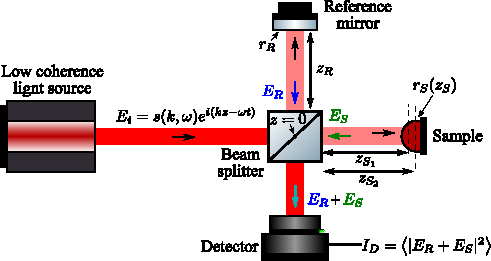
\includegraphics[width=.65\textwidth]{Figures/TheoreticalBasis/OCT_Model.pdf}
    \caption{Schematic of generic Michelson interferometer used in OCT.}
    \label{fig:OCT_Model}
\end{figure}

Interferometry measures the correlation between the electric fields of the light reflected by the sample and the reference mirror. Consider that the light source emits plane waves with electric field $E_i = s(k,\omega)e^{i(kz-\omega t)}$ at time $t$ and distance $z$ along the propagation axis, being $s(k,\omega)$ the complex amplitude, dependent on the angular frequency $\omega$ and wavenumber $k=2\pi / \lambda$ for wavelength $\lambda$. Assuming free space propagation and a 50/50 beam splitter, the reference beam propagates a distance $z_R$ from the beam splitter to the reference mirror with reflectivity $r_R$ and reflectance $R_R=|r_R|^2$, then reflected light propagates back to the beam splitter and its electric filed can be expressed as $E_R = \dfrac{E_i}{\sqrt{2}} r_R e^{i2kz_R}$.

On the other hand, light on the sample arm propagates a distance $z_S$ from the beam splitter to the sample. In biological tissues, the refractive index changes resulting in different reflectivities~\cite{}, therefore, the sample can be described as a discrete number $N$ of reflectors with reflectivities $r_{S_n}$ and reflectances $R_{S_n}=|r_{S_n}|^2$ located at distances $z_{S_n}$ as
\begin{equation}
    r_S(z_{S_n}) = \sum_{n=1}^N r_{S_n}\delta\left(z_S-z_{S_n}\right).
\end{equation}

\textbf{Coherent gating in OCT allows to reconstruct the function $\mathbf{\sqrt{R_{S_n}(z_{S_n})}}$ to produce images with optical contrast related to changes in the refractive index of the sample.}

Light backscaterred by the sample propagates back to the beam splitter with electric field $E_S=\dfrac{E_i}{\sqrt{2}}\sum\limits_{n=1}^Nr_{S_n}e^{i2kz_{S_n}}$. Reference and sample electric fields $E_R$ and $E_S$ interfere and a photodetector with responsivity $\rho$ captures the intensity producing a photocurrent $I_D(k, \omega)$ that can be described as
\begin{align}\label{eq:I_D(k,w)}
    I_D(k, \omega) &= \rho\left<\left|\frac{E_R}{\sqrt{2}} + \frac{E_S}{\sqrt{2}}\right|^2\right> \nonumber\\
    & = \rho\left<\left|\dfrac{E_i}{2} r_R e^{i2kz_R} + \dfrac{E_i}{2}\sum\limits_{n=1}^Nr_{S_n}e^{i2kz_{S_n}}\right|^2\right> \\
    & = \frac{\rho}{4}\left<\left|s(k,\omega) r_R e^{i2kz_R-\omega t} + s(k,\omega)\sum\limits_{n=1}^Nr_{S_n}e^{i2kz_{S_n}-\omega t}\right|^2\right>, \nonumber
\end{align}
assuming $z=0$ at the splitting surface of the beam splitter without loss of generalization, where $\left<\cdot\right>$ is the temporal averaging performed by the photodetector during the integration time of a single measurement, that is long enough to expect that $I_D$ is independent of the temporal component $\omega t$ given the fast temporal oscillation of light imposed by $\omega$. This is consequent with expansion of Eq.~\eqref{eq:I_D(k,w)} using $|E|^2 = E^*E$ that yields the spectral interferogram
\begin{align}\label{eq:I_D(k)}
I_D(k) &= \frac{\rho}{4}\left[S(k)\left(R_R + \sum_{n=1}^N R_{S_n}\right)\right] ... \nonumber\\
&+ \frac{\rho}{2} \left[S(k)\sum_{n=1}^N\sqrt{R_RR_{S_n}}\cos\left(2k\left[z_R-z_{S_n}\right]\right)\right] ... \\
&+ \frac{\rho}{4}\left[S(k)\sum_{n\neq m}^N\sqrt{R_{S_n}R_{S_m}}\cos\left(2k\left[z_{S_n}-z_{S_m}\right]\right)\right]. \nonumber
\end{align}
where $S(k) = |s(k,\omega)^2|$ is the light source spectrum and $z_R-z_{S_n}$ is the OPL difference.

There are three components in $I_D(k)$ as noted in Eq.~\eqref{eq:I_D(k)}. First one is a \textit{background} component that is independent of propagating distances and it is the largest component given that typically reference mirror reflectivity denominates the sample reflectivity. In general, this is a undesired component that is canceled out using background removal methods~\cite{}.

Second is a \textit{cross-correlation} component that depends on the spectrum of the light source $S(k)$, the wavenumber $k$ and the OPL difference $z_R-z_{S_n}$. This is the desired component in OCT imaging since it gives access to the sample reflectivity through the term $\sqrt{R_RR_{S_n}}$.

Last term is an \textit{auto-correlation} component that represents the interference between the different sample reflectors, independent of the reference light. This is commonly an artifact component that can be neglected increasing the magnitude of the other two components by increasing the reference mirror reflectivity.

Note that $I_D(k)$ in Eq.~\eqref{eq:I_D(k)} is the interference resulting from a particular wavenumber $k$, but the ultimate aim in OCT is to ``isolate'' the $\sqrt{R_RR_{S_n}}$ term along depth, that is related to OPL differences $z_R-z_{S_n}$. There are two approaches to retrieve the depth-dependent photoccurent $i_D(z)$, yielding two major OCT configurations: time domain OCT (TDOCT) and Fourier domain OCT (FDOCT). Also, note that depth-dependent signal $i_D(z)$ is given for a specific transverse point with coordinates $(x,y)$ of the sample. In raster scan systems, the beam is scanned in the sample plane using galvanometer scan mirror that deflects the light beam, and in each position $(x,y)$ an A-line is acquired. Given that the interest here so far is the axial scan, dependence on coordinates $(x,y)$ is omitted for simplicity.

\subsection{Time domain OCT}

Most straightforward way to obtain the depth-dependent signal is to use a mono-pixel detector to capture the interference while the reference delay $z_R$ is scanned by moving the reference mirror along the axial direction as shown in Figure~\ref{fig:TDOCT_Scheme}. The detector captures the intensity for all $k$ at the same time, thus $i_D(z_R)$ is the integration over all $k$ of $I_D(k)$, 
\begin{align}
    i_D(z_R) &= \frac{\rho}{4}S_0\left(R_R+\sum_{n=1}^N R_{S_n}\right)... \nonumber \\
    &+ \frac{\rho}{2}S_0 \sum_{n=1}^N \sqrt{R_RR_{S_n}} e^{-\left(z_R-z_{S_n}\right)^2 \Delta k^2}\cos\left[2k_0\left(z_R-z_{S_n}\right)\right].
\end{align}
where $S_0 = \int\limits_{0}^\infty S(k)dk$ is the spectral total power emitted by the light source, and a normalized Gaussian spectrum $S(k) =\dfrac{1}{\Delta k\sqrt{\pi}}e^{-\big[\frac{(k-k_0)}{\Delta k}\big]^2}$ is assumed, being $k_0$ the central wavenumber and $\Delta k$ the full-width at $1/e$ of the maximum.

\begin{figure}[htb!]
    \centering
    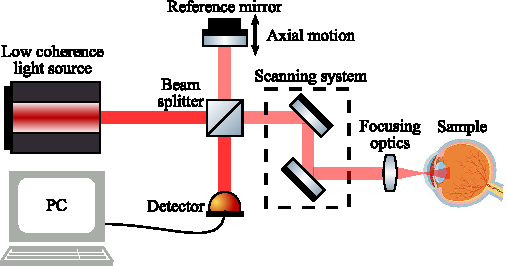
\includegraphics[width=.7\textwidth]{Figures/TheoreticalBasis/TDOCT_Scheme.pdf}
    \caption{Schematic of a generic TDOCT setup based on a Michelson interferometer, where axial scan is performed by displacing the reference mirror in the axial axis while recording the interference with a mono-pixel detector.}
    \label{fig:TDOCT_Scheme}
\end{figure}

Time domain A-line $i_D(z_R)$ consists of a background component (DC), proportional to $S_0$, and an interference component that is a summation of Gaussian functions with finite width, having peak-values of $\sqrt{R_RR_{S_n}}$ located at OPL differences $z_R-z_{S_n}$ and modulated by cosines of period $\pi/k_0$, equivalent to $\lambda_0/2$. $\gamma(z_R)=e^{-(z_R-z_{S_n})\Delta k^2}$ is known as the \textit{coherence function} and it causes a ``broaning'' of the interference signal of each reflector and its width is related to the coherence length of the light source that determines the axial resolution, thus $\gamma(z_R)$ is considered as the axial point-spread function (PSF). Figure~\ref{fig:Alines} illustrates a TDOCT A-line in Fig.\ref{fig:Alines}(b) for a sample characterized by three reflectors as shown in Fig.\ref{fig:Alines}(a).

\begin{figure}[htb!]
    \centering
    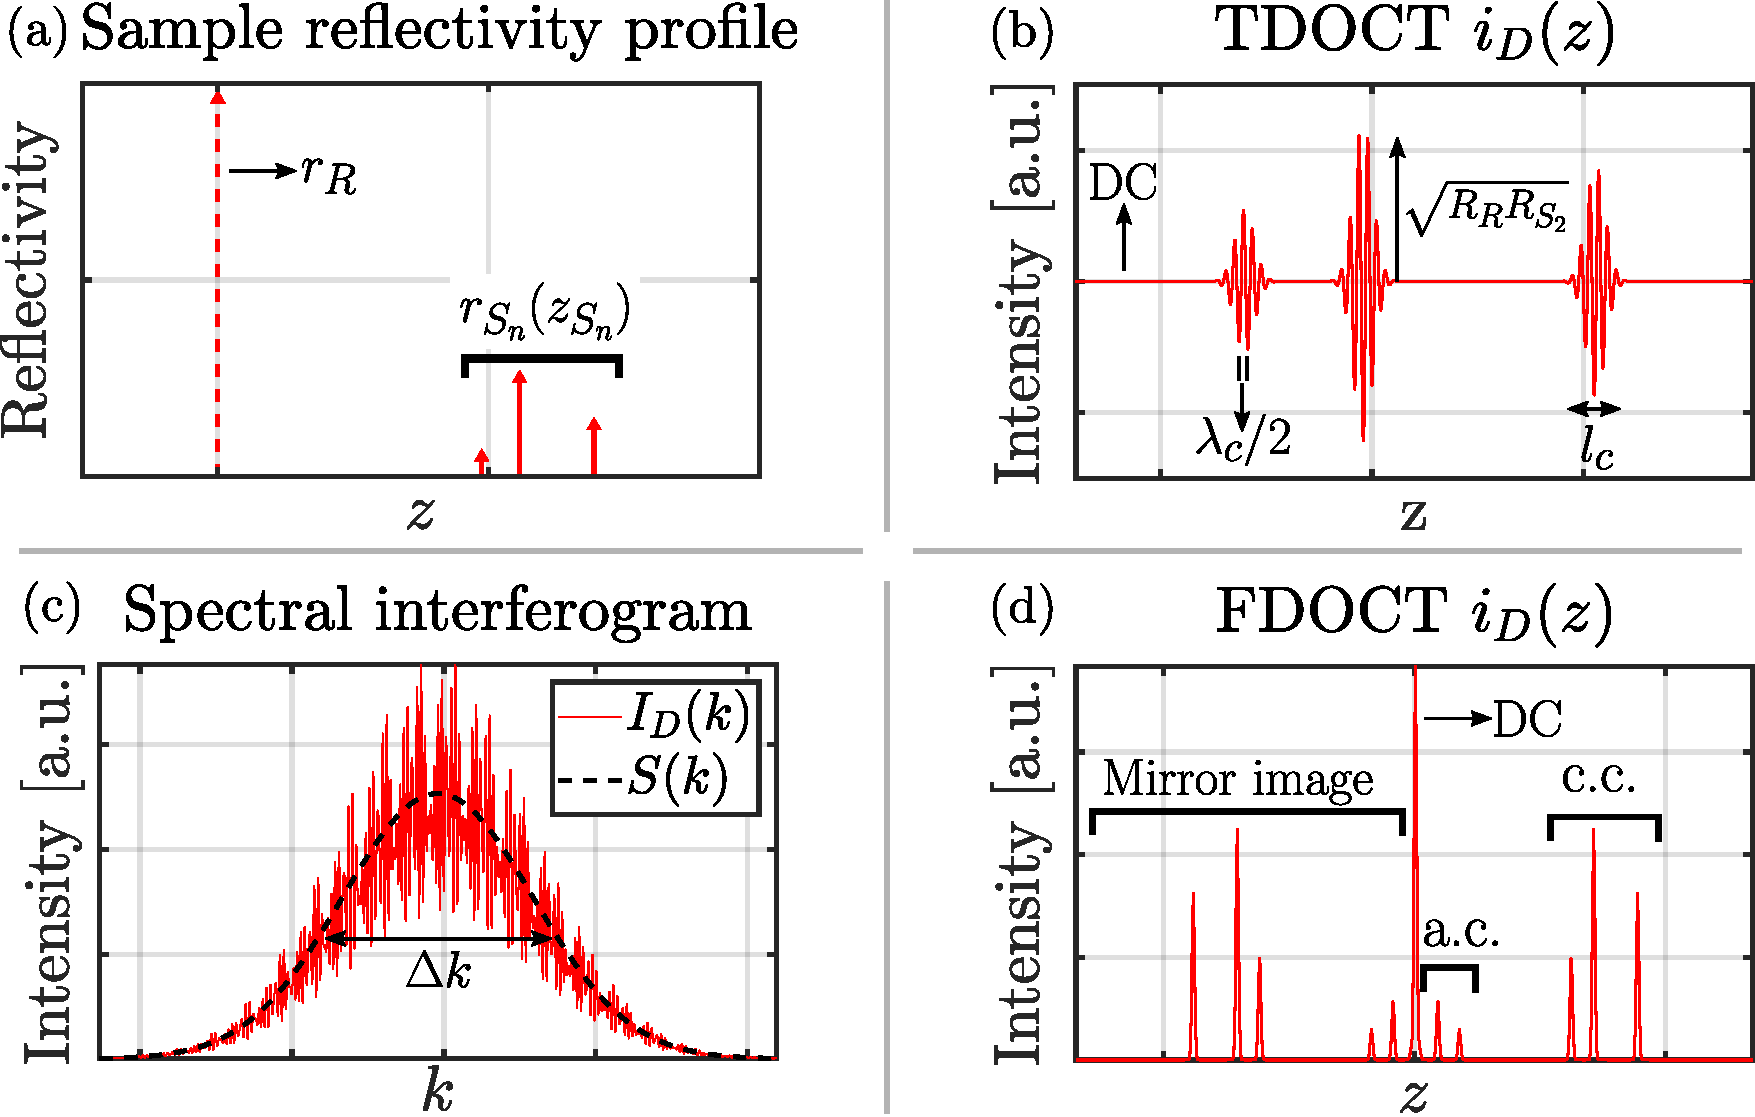
\includegraphics[width=.7\textwidth]{Figures/TheoreticalBasis/Alines.pdf}
    \caption{Illustration of A-lines obtained in OCT. a) Axial reflectivity profile for a sample characterized by three reflectors: b) TDOCT A-line, c) spectral interferogram and d) FDOCT A-line obtained as the Fourier transform of c), indicating the background (DC), cross-correlation (c.c.) and auto-correlation (a.c.) components.}
    \label{fig:Alines}
\end{figure}

Early OCT imaging systems including the first experimental demonstration of OCT in 1991~\cite{} employed a time domain detection. Designation of time domain arises from the fact that the reflectivity axial profile of the sample is acquired while displacing the reference mirror in time. This demands mechanical systems to displace the reference mirror and this limits imaging speed to A-line rates $<\sim$2~kHz, due to technical restrictions to develop precise fast motion systems with micrometric resolution and millimetric travel range. Furthermore, given that axial scan is acquired while the detector captures the signal at different times, stable systems are required to avoid artifacts during imaging due to changes of the imaging system, for instance, changes of the light source emission. By this reason, achievable sensitivity is limited, and this in addition to low imaging speed establish the major drawbacks of TDOCT.

\subsection{Fourier domain OCT}

Although TDOCT systems served well in early medical OCT development, their relatively slow scan rate and limited sensitivity restricted the potential of OCT and restricted its expansion to many medical applications. An improvement in sensitivity and imaging speed in OCT was possible with the introduction of FDOCT systems where the reference mirror remains fixed. Spatial and optical frequency domains are conjugate domains with the wavenumber and the OPL being Fourier transform duals. This concept led to development of Fourier domain acquisition where photocurrent $I_D(k)$ in Eq.~\eqref{eq:I_D(k)} is captured directly in the $k$ space and a subsequent Fourier transform $\text{FT}_k\left\{\cdot\right\}$ of the signal  along variable $k$ yields the depth-dependent photocurrent $i_D(z)$, with not need to displace the reference mirror.

Using the Fourier transform property $\text{FT}_k\left\{\cos(kz_0)\right\} = \frac{1}{2}\left[\delta\left(z+z_0\right) + \delta\left(z-z_0\right)\right]$, the convolution theorem $\text{FT}_k\left\{g\left(k\right)f\left(k\right)\right\} = \text{FT}_k\left\{g\left(k\right)\right\} \ast \text{FT}_k\left\{f\left(k\right)\right\}$, and the shifting property of delta functions $f(z)*\delta\left(z-z_0\right) = f(z_0)$, it is possible to obtain the FDOCT A-line $i_D(z) = \text{FT}_k\left\{I_D(k)\right\}$ from Eq.~\ref{eq:I_D(k)} as
\begin{align}\label{eq:i_D(z)}
    i_D(z) &= \frac{\rho}{8}\gamma\left(z\right)\left[R_R + \sum_{n=1}^NR_{S_n}\right] ... \nonumber\\
    &+ \frac{\rho}{4}\sum_{n=1}^N \sqrt{R_RR_{S_n}} \left[\gamma\left(2\left[z_R-z_{S_n}\right]\right) + \gamma\left(-2\left[z_R-z_{S_n}\right]\right)\right]...\\
    &+ \frac{\rho}{8}\sum_{n\neq m=1}^N \sqrt{R_{S_n}R_{S_m}} \left[\gamma\left(2\left[z_{S_n}-z_{S_m}\right]\right) + \gamma\left(-2\left[z_{S_n}-z_{S_m}\right]\right)\right], \nonumber
\end{align}
where again $\gamma\left(z\right)=\text{FT}_k\left\{S(k)\right\}$ is the coherence function of the source, that assuming a Gaussian emission spectrum is given by
\begin{align} \label{eq:SGamma}
    S(k) =\frac{1}{\Delta k\sqrt{\pi}}e^{-\big[\frac{(k-k_0)}{\Delta k}\big]^2} \xleftrightarrow{\hspace{8 pt}\text{FT}\hspace{8 pt}} \gamma(z) = e^{^{-z^2\Delta k^2}}.
\end{align}

Eq.~\eqref{eq:i_D(z)} contains three components as Eq.~\eqref{eq:I_D(k)}; background, cross-correlation and auto-correlation components. Figure~\ref{fig:Alines} shows an example of a Fourier domain A-line in Fig.~\ref{fig:Alines}d) for a sample with three reflectors as shown in Fig.~\ref{fig:Alines}a) and its corresponding interferogram in $k$ space in Fig.~\ref{fig:Alines}c). Cross-correlation component provides access to the signal of interest in OCT $\sqrt{R_RR_{S_n}}$ by each reflector appearing at positions $\pm2(z_R-z_{S_n})$ and being ``broadened'' by the coherence function similarly to the case of the TDOCT A-line. The apparent position of the reflectors $\pm2(z_R-z_{S_n})$ have a factor of 2 since the interferometer measures the round-trip distance.

There is a ``mirror image'' produced by the fact that $I_D(k)$ is real, hence its Fourier transform is Hermitian symmetric, that is, the positive values are the complex conjugate of the negative values, and this is represented in the double sign of $\pm2(z_R-z_{S_n})$. This does not have an important influence if the sample is positioned entirely in one side of the zero OPL, such that it is possible to extract only one half of the Fourier spectrum to avoid the mirror image.

Background component appears as a large component centered at the zero OPL. In general, it can be easily omitted from the signal since the reflectors of the sample are positioned beyond the zero OPL such that cross-correlation terms do not overlap with the background component. However, additional to the main lobe, side lobes may appear and cause significant artifacts overlapping with the cross-correlation terms, therefore, background is typically removed by recording the spectrum of the source blocking the light from the sample arm and then subtracting this background spectrum to every measurement.

Autocorrelation component appears near the zero OPL if the position of the reference mirror is such that $(z_{S_n}-z_{S_m}) << (z_R-z_{S_n})$, and this way it is possible to omit this artifact, but a more direct solution is to adjust the reference reflectivity to ensure that amplitude of cross-correlation terms are much higher than amplitude of auto-correlation terms.

Sensitivity improvement in FDOCT with respect to TDOCT arises from the fact that interference for all depths are captured simultaneously, considering that the signal is acquired in $k$ space and it is known that each value in frequency domain contributes to all values in spatial domain. In FDOCT, there are two approaches to measure the spectral interferogram. Most intuitive way is to use a digital spectrometer as detector as shown in Figure~\ref{fig:SDOCT_Scheme}, which provides the intensity signal as a function of wavenumber $I_D(k)$ in a single measurement, and it is known as spectral domain OCT (SDOCT). Digital spectrometers are composed of a linear camera and an optical system that separates the spectral components of input light in such way that each pixel of the detector captures the intensity of a portion of the spectrum. Imaging speed in SDOCT is limited by acquisition rate of the linear camera and typical A-line rates are between 2 -- 50~kHz.

\begin{figure}
    \centering
    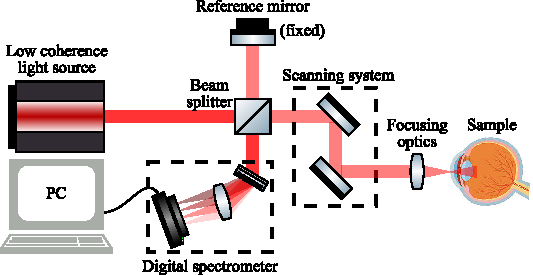
\includegraphics[width=.75\textwidth]{Figures/TheoreticalBasis/SDOCT_Scheme.pdf}
    \caption{Schematic of a generic SDOCT setup based on a Michelson interferometer, where axial scan is obtained by computing the Fourier transform of the spectral interferogram acquired with a digital spectrometer.}
    \label{fig:SDOCT_Scheme}
\end{figure}

The second approach in FDOCT is to use a tunable light source with a narrow spectrum and to acquire the interference signal $I_D(k)$ with a single-element photodetector while the central emission wavenumber $k$ of the light source is swept among a broad spectrum, and it is known as wavelength-swept source OCT (SSOCT). It is also referred as optical frequency domain imaging (OFDI) instead of low coherence interferometry given that, in rigorous terms, instantaneous emission of the tunable light source is considered coherent. OFDI achieves the highest imaging speed in OCT, presenting A-line rates up to 200~kHz, and it is limited by the sweeping rate of the light source. Hereafter, OFDI is used to refer to the imaging technique and SSOCT is used to refer to the OCT systems used for OFDI. A more detailed description of SSOCT systems is provided below, because this is the one of interest for this work.

\subsection{Optical frequency domain imaging}

Operation of OFDI is grounded on the fact that OPL and wavenumber are conjugate variables. In low coherence interferometry, interference is acquired illuminating the sample with light spanning several wavenumbers while OPL is scanned. In the alternative scenario, interference corresponding to all OPLs at the same time is acquired while illuminating the sample with light spanning a single wavenumber that is scanned, and this is the principle of operation of OFDI. Then, a Fourier transform of the signal in spectral domain yields the depth-dependent signal.

Detection scheme in OFDI employs a single-element detector, allowing higher A-line rates than in SDOCT systems that are limited by the acquisition rate of the linear camera, which is composed of multiple pixels. Increasing imaging speed reduces motion artifacts when imaging in vivo and allows larger scans in limited time. Tunable light sources are available in the 1--1.3~$\mu$m wavelength range, where cameras technology is not well established, hence SSOCT systems are used commonly in the 1--1.3~$\mu$m range that serves for multiple medical applications and SDOCT in the complementary 0.85--1~$\mu$m range used mainly in ophthalmology.

The most relevant specifications of tunable light sources in SSOCT are repetition rate, instantaneous linewidth $\delta\lambda$, tunable range $\Delta\lambda$ and tuning curve $k_i(t)$. Axial resolution is determined by central wavelength of emission $\lambda_c$ and tunable range $\Delta\lambda$ equally to Eq.~\ref{eq:axialRes}, $\delta_z = \frac{2\ln 2}{\pi}\frac{\lambda_c^2}{\Delta\lambda}$, thus it is independent of instantaneous linewidth. Instead, the depth range $\Delta z$ observed within a single A-line is determined by the instantaneous linewidth as
\begin{align}
\Delta z = \dfrac{\lambda_c^2}{4\delta\lambda}
\end{align}
and is independent of tunable range. Note that central wavelength mediate in both parameters. As a numerical example, a tunable light source with instantaneous linewidth $\delta\lambda=0.1$~nm and tunable range $\Delta\lambda=125$~nm centered at $\lambda_c=1.3~\mu$m provides $6~\mu$m axial resolution along $4.2$~mm depth range. The same light source but with central wavelength $\lambda_c=860$~nm provides $2.7~\mu$m axial resolution over $2.15$~mm.

Tunable curve $k_i(t)$ determines the instantaneous wavenumber as a function of time $t$. Ideally, this is a linear curve $k_i(t) = k_0 + k_st$ where $k_0$ is the initial wavenumber and $k_s$ is the wavenumber step between consecutive instantaneous wavenumbers. In practice, $k_i(t)$ is a non-linear function of time and thus linearization is required, typically performed on post-processing prior to computing the Fourier transform of the spectral interferogram, otherwise, artifacts appear degrading axial resolution.

Development of SSOCT systems have inherited technology from optical communications in the near infrared spectrum that employs similar optical components such as tunable laser sources, optical fiber and detectors. In that sense, there are multiple types of tunable light sources relying on different principles of operations, but currently the development of fast, stable, linear, low-cost tunable light sources is a very active area of research.

Lasers are optical oscillators comprising a gain medium that is pumped optically or electrically to amplify light by stimulated emission, and an optical cavity that gives coherent optical feedback for laser oscillations~\cite{}. Semiconductor optical amplifier (SOA) is a gain medium widely used for tunable lasers because they offer a high gain in a broad bandwidth, a rapidly response time, in the picosecond scale, and a wide range of gain center wavelengths depending on the semiconductor materials. One way to construct tunable lasers is to incorporate in the basic laser instrumentation an internal or external scanning filter to select the central wavelength of the instantaneous emission. One of the first approaches developed for OCT applications was tunable laser based on scanning filter using a polygonal mirror and to date this is widespread in research and medical systems. Polygon-based tunable lasers offer high sweep rate in a wide tuning range with narrow linewidth, ideal features for OCT imaging.

In polygon-based lasers, the optical cavity includes a diffraction grating, a telescope and a rotating polygonal mirror with tens of facets. Light emitted by a SOA within a broad spectrum is reflected by the diffraction grating in such way that there is an angular separation of spectral components. Light is relayed to the polygonal mirror through the telescope, and only the spectral component incident perpendicular to the mirror surface is reflected back to the grating and then to the SOA, proving a coherent light feedback. Rotation of the polygonal mirror changes surface angle and therefore the instantaneous spectral component that has perpendicular incidence also changes. Drawbacks of this scanning filter approach is that polygonal mirror is a relatively bulky and moving part.

Figure~\ref{fig:SSOCT_Scheme} illustrates an optic fiber-based SSOCT system using a polygon-based tunable laser. Light from the tunable laser is delivered to an optic fiber beam splitter that divides the light into the sample and reference arms, then, reflected light from both produce interference that is detected by a photodetector and digitized. In this scheme, balanced detection is illustrated using two detectors to subtract the background signal and thus suppressing excess noise. Moreover, SSOCT systems require a trigger signal to synchronize detector acquisition with rotation of the polygonal mirror. In the system of Fig.~\ref{fig:OFDI_Scheme}, the trigger signal is generated by a narrowband fiber Bragg grating (FBG) that reflects light of a specific wavelength, thus when the laser source emits this wavelength, the FBG reflects light generating a pulse that indicates the beginning of interferogram acquisition, performed using N analog-to-digital conversions (ADC) following a sample clock.

\begin{figure}[htb!]
    \centering
    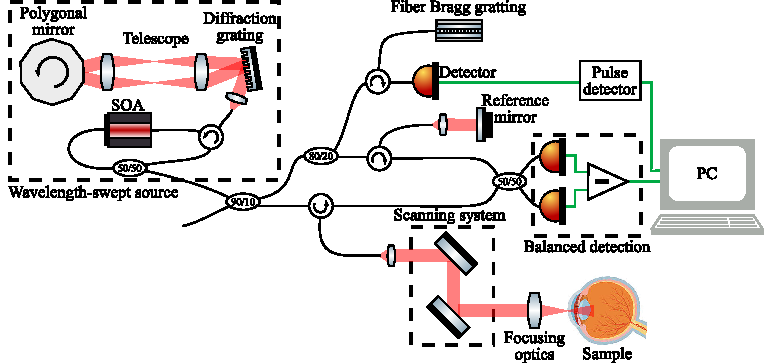
\includegraphics[width=\textwidth]{Figures/TheoreticalBasis/SSOCT_Scheme.pdf}
    \caption{Schematic of a fiber-based SSOCT setup where the wavelength-swept source changes its instantaneous central wavelength in time due to the rotation of the polygonal mirror. A trigger signal to start the acquisition of the spectral interferogram is produced by the fiber Bragg grating that is designed to reflect a single wavelength, indicating the start of a sweep cycle of the light sorce.}
    \label{fig:SSOCT_Scheme}
\end{figure}

Compact tunable lasers have been possible with vertical cavity surface emitting lasers (VCSEL) in conjunction with a micro-electro-mechanical mirror system (MEMS) used to vary the cavity length of the VCSEL, thereby tuning the output wavelength. MEMS-VCSEL sources however have a limited tuning range and broad instantaneous linewidth although they are in current development to provide a powerful alternative to polygonal-based sources~\cite{}. In addition, current research focuses in developing akinetic tunable lasers to provide more robust and reliable light sources with the same or even better features of polygon-based sources~\cite{}.

\subsection{Phase stability in OCT configurations}

Being an interferometric technique, OCT provides information of the \textit{complex amplitude} of the light backscattered by the sample, and this includes phase and amplitude information. This is an important feature of OCT because the complex amplitude provides more information than the amplitude (or intensity) alone, enabling operation of phase-resolved functional techniques and phase-dependent post-processing.

In OCT, there are several undesired contributions to the phase that are considered as \textit{phase noise}, arising from the system or from the sample, making development of phase-resolved OCT technology challenging. The ability of a system to provide repeatable phase measurements is known as \textit{phase stability} and it exists when there is a constant phase relation between measurements, that is, when the phase difference between entirely correlated measurements is zero. In phase sensitive techniques like flowmetry, phase difference between successive measurements is directly related to the flow velocity, and phase stability is crucial because phase noise causing phase fluctuations adds spurious contribution to the calculation of the phase difference inducing errors in the velocity estimation.

Phase stability is greatly influenced by the configuration used for axial and transverse scan. In SDOCT, the parallel acquisition of the entire spectral interferogram within a single measurement ensures phase stability inside A-lines, thus axial axis is phase stable. In addition, the high repeatability of spectrometers ensure phase stability along successive A-lines measured at different times while scanning the beam in the sample, hence in principle SDOCT provides three-dimensional phase stability. However, there are two additional sources of phase noise in OCT, one induced by sample motion that is detailed in Section~\cite{sec:phaseStab}, and second is induced in the galvanometer scanning system, due to separation of the pivot position of each galvanometer mirror and the back focal plane of the scan lens that adds a phase offset depending on the instantaneous angle of the mirror. Although there is a physical limitation in positioning the pivot point of both galvanometers mirrors at the back focal length of the scan lens, precise alignment of one mirror would ensure phase stability along its corresponding lateral scan axis.

In SSOCT systems, achieving phase stability have been more challenging than in SDOCT because each component of the spectral interferogram is acquired sequentially in time and not in parallel like in a spectrometer. In principle, this is not a limitation if experimental conditions of the system during A-line acquisition do not change, but there is a particular issue in regard to the trigger signal that have a detriment effect in phase stability. SSOCT systems require a trigger signal to synchronize A-line acquisition with wavelength sweep of the light source, for instance using a Fiber Bragg grating like in Fig.~\ref{fig:SSOCT_Scheme}. However, the fast sweeping cycle of the light source demand precise electronics to obtain a perfect synchronization, but in practice this is not the situation and there is a time delay or \textit{jitter} in the sample clock for acquisition with respect to the trigger signal. as a consequence, acquisition starts arbitrarily within the sweep cycle of the light source.

A jitter in synchronization causes a shift $\delta k$ in the acquired spectral interferogram, thus the measured signal is $\tilde{I}_D(k) = I_D(k-\delta k)$. Depth-dependent signal obtained as $i_D(z)= \text{FT}_k\{\tilde{I}_D(k)\}$ results in
\begin{align*}
    \tilde{i}_D(z) &= \text{FT}_k\{I_D(k-\delta k)\} \nonumber \\
    &=  \text{FT}_k\{I_D(k)\} e^{-i2\pi z\delta k} \nonumber \\
    &=  i_D(z) e^{-i2\pi z\delta k}
\end{align*}
being $i_D(z)=\text{FT}_k\{I_D(k)\}$ the unmodified depth-dependent A-line. Note that effect of spectral shift only impacts the phase of the A-line by the factor $e^{-i2\pi z\delta k}$ that represents a phase ramp with slope $-2\pi\delta k$, known as \textit{phase jitter} noise, but the amplitude $|\tilde{i}_D(z)|=|i_D(z)|$ remains unchanged, thereby traditional structural OCT image based on the intensity $|\tilde{i}_D(z)|^2=|i_D(z)|^2$ is not affected. The random behavior of jitter in synchronization causes that the spectral shift $\delta k$ varies randomly between spectral interferograms, and this dramatically impacts phase stability in raster scan systems because A-lines are captured sequentially in time while displacing the beam in the sample plane, inducing spatially-varying phase-jitter noise.

An approach to avoid phase-jitter is the use of $k$-clocks that produce a sample clock linear in $k$ using a Mach-Zehnder interferometer. In standard systems, signal acquisition is performed linearly in time with $N$ ADC following an internal electronic sample clock. With a $k$--clock, ADC are performed linearly in $k$ with certainty. Therefore, the use of a $k$--clock avoids phase-jitter because the uncertainty in trigger signal is solved, at the same time that acquired signal is linear in $k$ eliminating the need of signal linearization in post-processing. Although there are $k$-clocked SSOCT systems available, they are not widespread because the need of additional hardware, thus phase-jitter is a very common issue affecting standard research and medical OCT systems. However, even using a $k$-clock, SSOCT systems are sensitive to galvanometer and sample motion phase noise, affecting its phase stability.

In the previous descriptions, it is possible to note that phase stability is very limited in raster scan systems, whether SDOCT or SSOCT, because transverse scan is performed in time. Parallel acquisition of A-lines for different transverse location can be achieved with extended-field systems where light is projected onto the sample in an extended area. In line-field SDOCT (LF-SDOCT), the sample is illuminated with a line-shaped beam produced by a cylindrical lens and the linear detector in the digital spectrometer is replaced by a two-dimensional detector; one dimension correspond to the $k$ space and the orthogonal dimension corresponds to the transverse fast scan axis. Hence, a single acquisition of the detector provides a B-scan view, and a single galvanometer is required to scan the beam along the slow scan axis providing three-dimensional images. Parallel acquisition along fast scan axis ensures phase stability in vivo in this axis as long as acquisition rate is relatively fast compared to the velocity of the sample motion, nonetheless, slow scan axis typically remains phase unstable.

TDOCT and SSOCT systems allow full field (FF) acquisition where the sample is illuminated with an extended collimated beam, the single-element detector is replaced by a two-dimensional detector and additional optical lenses are used to image the sample plane on the detector plane, hence a single axial scan provides an entire tomogram with volumetric phase stability, even in vivo if acquisition rate is relatively fast compared to the velocity of the sample motion. Figure~\ref{fig:LF_FFOCT_Scheme} illustrates simple schematics of LF-SDOCT and FF-SSOCT systems.

\begin{figure}
    \centering
    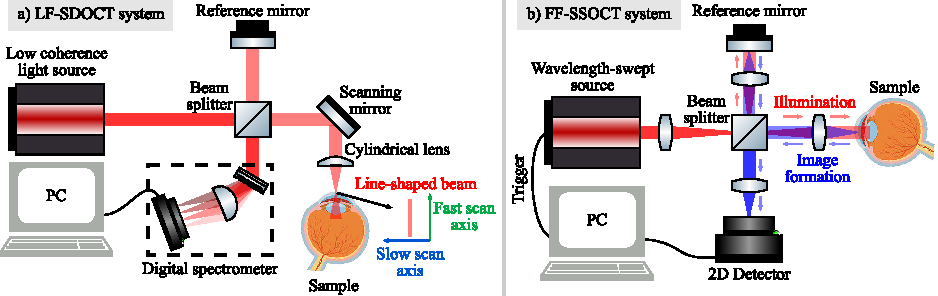
\includegraphics[width=\textwidth]{Figures/TheoreticalBasis/LF_FFOCT_Scheme.pdf}
    \caption{Schematic of generic a) LF-SDOCT setup for acquisition of a B-scan in a single detector shot and b) FF-SSOCT setup for acquisition of a tomogram in a single cycle of the wavelength-swept source. Red path illustrates the illumination beam and blue path the image formation on detector plane for a point.}
    \label{fig:LF_FFOCT_Scheme}
\end{figure}

Extended-field OCT systems are custom configurations used in particular scenarios, like in the CAC research area because they offer sufficient phase stability, but they are not widespread given that they have a more complex optical design including 2D detectors that are not well developed in terms of speed and sensitivity in the near-infrared range, but more importantly, they are more prone to multiple scattering. Scattered light in tissue can be divided into two components: single scattering and multiple scattering (MS), the former is the backscattered signal of interest in OCT and the latter is an undesired component arising from light that is scattered multiple times following random paths that reaches the detector, but it does not contribute direct information to the OCT signal due to its random properties. Raster scan systems have an intrinsic rejection to MS given because of confocal gating, that is, the focused beam scans a small region of the sample in a limited field of view (FoV). Extended detection is more prone to collect MS photons given that the FoV during each measurement is larger.

\section{Modelling the acquisition of the complex OCT signal}\label{Model}

In previous section, OCT experiment was described and analyzed from an interference perspective to derive the acquisition of axial scan that provides the depth-dependent signal by means of optical interferometry, however, this corresponds to the complex field of backscattered light by the sample but the ultimate aim is to obtain the \textit{scattering potential} of the sample denoted as $\eta$ that gives information of sample structure. In other words, in OCT the optical beam probe is used to measure $\eta$ indirectly; the acquired signal contains the sample scattering information as well as the effect of the optical system. In the ideal situation, the effect of the optical system is not significant and the measured signal is directly related to $\eta$. This is the case of systems with aberration-free optical beams where imaging is diffraction-limited and the theoretical lateral resolution is achievable, but in the presence of aberrations, the optical field is distorted and effective lateral resolution is reduced.

Scattering theory can be used to derive a model of the imaging formation process that relates the measured signal with the sample structure, known as \textit{forward model}. Inversion of the forward model results in the \textit{inverse scattering model} that allows to recover an approximate sample structure from the backscattering signal. Solutions to the inverse scattering model brought the development of computational techniques for aberration correction of OCT tomograms. In this section, the forward model is presented and subsequent section surveys solutions to the inverse scattering model to correct aberrations in post-processing.

\subsection{Confocal gating for lateral scan in OCT}

In raster scan systems, the transverse scan is performed using confocal gating resulting from the distribution of the focused beam. When light is focused on the sample plane, the illuminated cross-sectional area defines the lateral resolution and it can be given in terms of the beam diameter. Typically, at the back focal length of the optical system, the probe beam with central wavelength $\lambda_c$ is a Gaussian beam with a $1/e^2$--diameter $D$, and after the optical system, light is focused at the front focal length $f$ in a spot with a $1/e^2$--radius $w_0$ that defines the diffraction-limited lateral resolution $\delta x$
\begin{align}
    \delta x = 2w_0 = \frac{4\lambda_c}{\pi} \frac{f}{D},
\end{align}
where $\dfrac{D}{2f} = \text{NA}$ is the numerical aperture of the optical system, and its inverse relation to $\delta x$ means that fine transverse resolution can be obtained in high NA systems that produce small focused spots. Due to convergence and divergence, the $1/e^2$--radius $w(z)$  of the focusing beam varies with depth $z$, and setting $z=0$ at the front focal plane, $w(z)$ can be expressed as
\begin{equation}\label{eq:beamWaist}
    w(z) = w_0 \sqrt{1 + \left(\frac{z\lambda_c}{\pi w_0^2n}\right)^2}
\end{equation}
where $n$ is the refractive index of the propagating medium.

Eq.~\ref{eq:beamWaist} shows that diffraction-limited resolution is only possible at the focal plane ($z=0$) and is degraded for other planes. However, for distances $z$ relatively close to the focal plane, change of spot size is relatively small. The confocal parameter $b$ is defined as the distance within which the spot size is smaller than $\sqrt{2}\delta x$ and thus resolution can be considered as nearly constant, and it is given by
\begin{equation}
    b = 2z_R = \frac{\pi\delta x^2}{\lambda}
\end{equation}
where $z_R$ is known as the Rayleigh range. Confocal parameter defines the region where defocus is negligible and is also referred to as depth of field (DoF). It is proportional to the beam spot size squared and this establishes the lateral-resolution--DoF trade-off; high NA systems provides high resolution images in a limited DoF whereas low NA systems provides low resolution images in an extended DoF. In general, OCT systems employs low NA (between 0.01 and 0.15) to obtain tomograms with nearly focal resolution throughout the whole axial scan and this have limited transverse resolution in OCT to $\sim>10~\mu$m, although in certain applications high NA systems are used and known as optical coherence microscopy (OCM)~\ref{}.

To illustrate confocal gating and its relation to numerical aperture, Figure~\ref{fig:ConfocalScan}a) shows the focused beam produced by two optical systems in different NA regimes, for a wavelength $\lambda_c = 1~\mu$m. Low NA system (red) produces a large spot size but its size remains nearly constant along a large DoF. In contrast, the second system (blue) has a NA four times larger producing a spot size four times smaller but its size increases abruptly reducing the DoF by $4^2$ times. Fig.~\ref{fig:ConfocalScan}b) shows the square relationship between confocal parameter and transverse resolution, indicating the corresponding values of the NA used in Fig.~\ref{fig:ConfocalScan}a).

\begin{figure}[htb!]
    \centering
    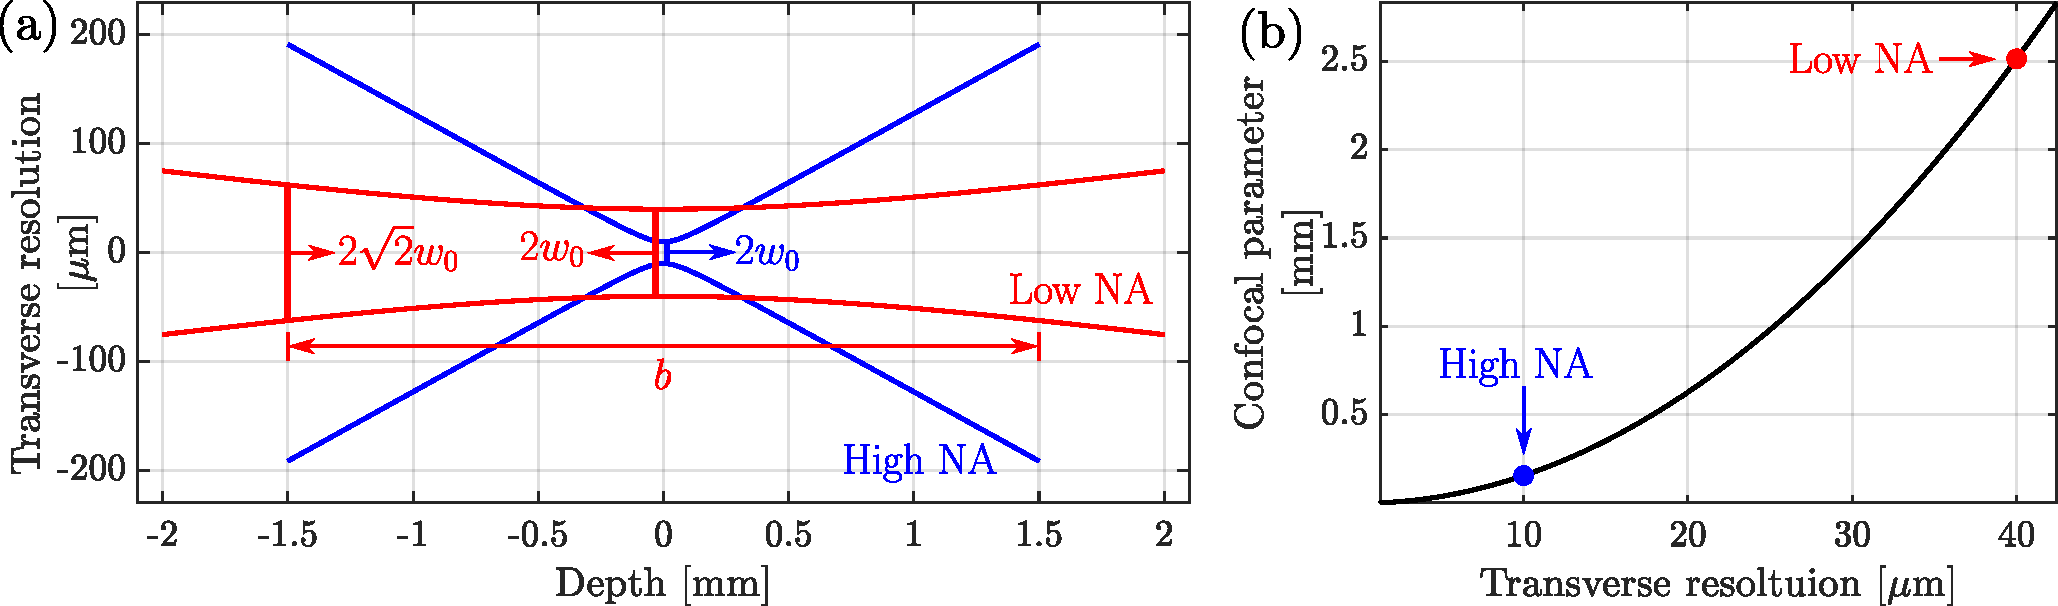
\includegraphics[width=\textwidth]{Figures/TheoreticalBasis/ConfocalScan.pdf}
    \caption{Illustration of confocal gating for light with $\lambda_c = 1\mu$m. a) Focused beam produced by two optical systems with relatively low and high NA. b) Relation between confocal parameter and transverse resolution.}
    \label{fig:ConfocalScan}
\end{figure}

With this qualitative description of the resolution-DoF--trade-off, it is possible now to analyze how this impacts the acquired complex signal.

\subsection{Forward model}

This section presents the forward model (FM) that relates the measured OCT signal to the sample structure considering the effect of the optical system using a model for the image formation process. In the FM, the propagation of the Gaussian probe beam is taking into consideration to derive an expression for the interference signal that also considers the effect of confocal scan. From Fourier optics theory, the acquired signal $S(x,y; k)$ for wavenumber $k$ at transverse coordinates $(x,y)$ can be modelled as $S(x,y; k)= h(x,y,z; k)\otimes\eta(x,y,z)$, that is the convolution (denoted by $\otimes$) of the system point-spread function (PSF) $h(x,y,z; k)$ with the scattering potential of the sample $\eta(x,y,z)$~\ref{},
\begin{equation}\label{eq:conv}
    S(x,y; k) = \iiint h(x-x', y-y', z'; k) \eta(x',y',z') \text{d}x' \text{d}y' \text{d}z'
\end{equation}
where the integration over $z'$ indicates that light is captured simultaneously for all depths, as occurs in Fourier domain detection. The PSF $h(x,y,z; k)$ can be expressed as the product of the incident and detection complex probe beams $g_i(x,y,z;k)$ and $g_d(x,y,z;k)$ respectively, but given that OCT is based on a reflection (double-pass) geometry, the incident and collection beams are identical to $g(x,y,z;k)$, hence
\begin{equation}\label{eq:PSF1}
    h(x,y,z; k) =k^2|A(k)|^2g^2(-x, -y, z; k),
\end{equation}
where $|A(k)|^2$ is the power spectral density and the inversion of lateral coordinates $(x,y)$ is due to the reflection geometry.

To derive a model for the probe beam $g(x,y,z;k)$, consider that the beam at the focal plane $z=z_0$ and transverse coordinate $\mathbf{r_0} = (x,y,z_0)$ is a normalized Gaussian probe beam
\begin{equation}\label{}
    g_0(\mathbf{r_0}; k) = \frac{1}{2\pi w_0^2(k)}e^{-\mathbf{r_0}^2/[2w_0^2(k)]},
\end{equation}
with waist radius $w_0(k) = \alpha / k$ for wavenumber $k$ and $\alpha = \pi/\text{NA}$. Using plane-wave decomposition with transverse frequency coordinate $\mathbf{q} = (q_x, q_y, 0)$, the beam at $\mathbf{r} = (x, y, z)$ in any plane $z$ is described as
\begin{equation}\label{}
    g(\mathbf{r}; k) = \frac{1}{(2\pi)^2} \iint e^{i(z-z_0)\sqrt{k^2 - q^2}} e^{-q^2\alpha^2/2k^2} e^{i\mathbf{q}\cdot\mathbf{r}} \text{d}^2q
\end{equation}

Using Eqs.~\ref{eq:conv} and \ref{eq:PSF1}, it is possible to model the measured OCT interference signal taking into consideration the beam distribution, as explained in detail in Ref.~\ref{}, by means of the expression
\begin{equation}\label{eq:FM}
    S(\mathbf{r'}; k) = \frac{A(k)}{(2\pi)^2 k} \iiint f^2(\mathbf{r}-\mathbf{r'}; k) \eta(\mathbf{r}) \text{d}^2r \text{d}z,
\end{equation}
where the term $f^2(\mathbf{r}; k)$ is given by
\begin{equation}\label{eq:f^2}
    f^2(\mathbf{r}; k) = \frac{1}{8\pi^2}\left(\frac{\alpha^2}{k^2}+\frac{iz}{k}\right)^{-1} \iint e^{-q^2\alpha^2/4k^2} e^{iz\sqrt{4k^2-q^2}} e^{-i\mathbf{q}\cdot \mathbf{r}} \text{d}^2q.
\end{equation}

To understand Eq.~\ref{eq:FM}, note that $\mathbf{r'}=(x',y',z_0)$ is the instantaneous transverse position of the probe beam during a raster scan. The signal $S(\mathbf{r'},k)$ measured for the instantaneous wavenumber $k$ when the beam is located at the instantaneous position $\mathbf{r'}$ \textbf{is the contribution of all point scatterers in the sample weighted by the function $f^2(\mathbf{r}-\mathbf{r'}; k)$}, and scaled by a value proportional to the light source intensity for k, $A(k)$. Finally, a Fourier transform of $S(\mathbf{r'}; k)$ with respect to $k$ yields the depth-dependent signal $S(\mathbf{r'}, z)$. In regard to $f^2(\mathbf{r}-\mathbf{r'}; k)$, the factor $\frac{1}{8\pi^2}\left(\frac{\alpha^2}{k^2}+\frac{iz}{k}\right)^{-1}$ can be considered as a depth-dependent signal-loss factor that describes the signal reduction far from the focal plane, $e^{-q^2\alpha^2/4k^2}$ is related to the Fourier spectrum of the Gaussian beam, the factor $e^{iz\sqrt{4k^2-q^2}}$ encompasses both the interference and the PSF broadening effect, responsible of the signal blurring, and last factor $e^{-i\mathbf{q}\cdot \mathbf{r}}$ is the Fourier transform kernel as Eq.~\ref{eq:f^2} is actually a Fourier integral.

To illustrate the forward model, Figure~\ref{fig:FM1} shows an example of an OCT B-scan image simulated using Eq.~\ref{eq:FM}. For this purpose, a collection of $128$ point scatterers with random positions where defined within an axial and lateral field of view (FoV) of $820\times 450~\mu$m as depicted in Fig.~\ref{fig:FM1}a). The light source have $\Delta\lambda=150$~nm and $\lambda_c=1.310~\mu$m providing an axial resolution of $\delta z=5~\mu$m. The numerical aperture is NA $= 0.25$, a relatively high value, resulting in lateral resolution $\delta x=5~\mu$m throughout a depth of field of $b=30~\mu$m, producing the Gaussian beam shown in Fig.~\ref{fig:FM1}b), where the focal plane is clearly located at $z_0=0$. To generate the simulated OCT image shown in Fig.~\ref{fig:FM1}c), the location of the Gaussian beam is changed iteratively, and in each location the contribution of all point scatterers weighted by $f^2(\mathbf{r}-\mathbf{r'}; k)$ is computed using Eq.~\ref{eq:FM}. At the $n$-th iteration, the location of the Gaussian beam is $\mathbf{r}'_m=(n\text{d}x - \frac{\Delta x}{2},0,z_0)$, where $\Delta x$ is the lateral FoV and $\text{d}x = 1.75~\mu$m is the sampling step which is smaller than Nyquist sampling $\delta x / 2$.

\begin{figure}[htb!]
    \centering
    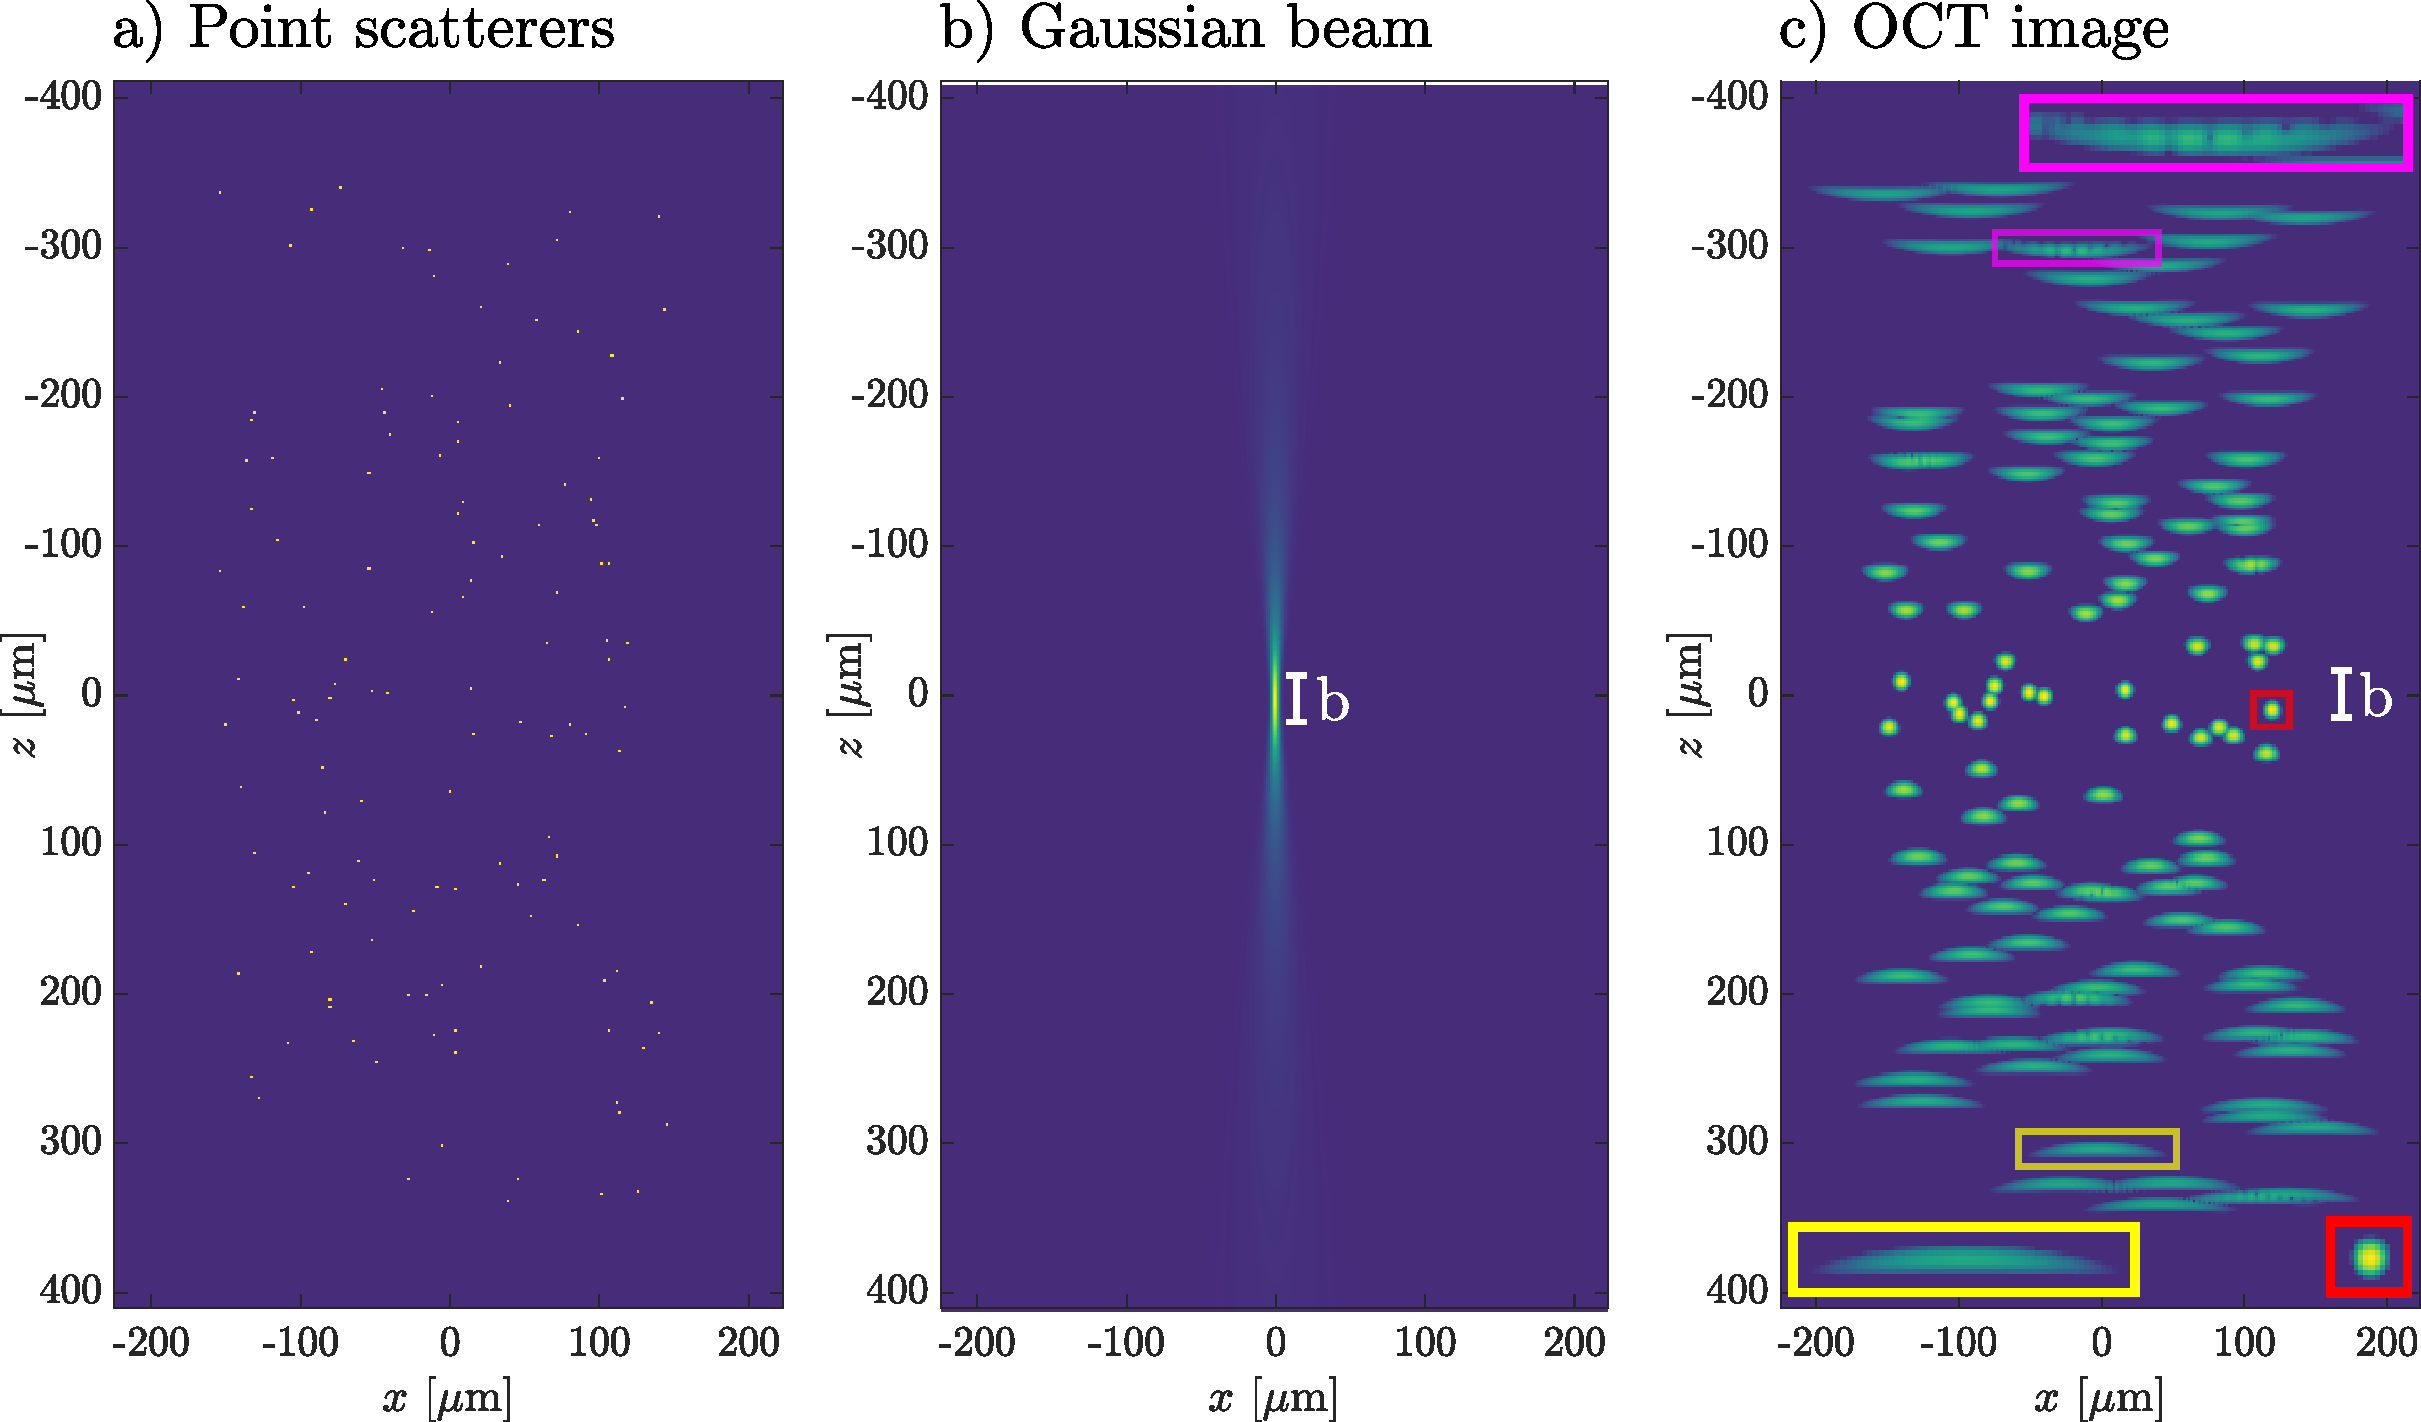
\includegraphics[width=\textwidth]{Figures/TheoreticalBasis/FM.pdf}
    \caption{Simulation of an OCT image in high-NA regime. a) Sample consisting of randomly located point scatterers, b) Gaussian beam of the system with NA$=0.25$ and c) OCT image simulated using the forward model, displayed in logarithmic scale.}
    \label{fig:FM1}
\end{figure}

The lateral blurring due to the convergence and divergence of the probe beam is evident in Fig.~\ref{fig:FM1}c). Resolution within the confocal region marked as $b$ is diffraction-limited, so that point scatterers inside $b$ appear in focus, like the one inside the red rectangle, contrary to point scatterers away from the focal plane that appear blurred in the lateral axis as a consequence of beam size increase, such as the one in the yellow rectangle. Note that superposition of signal from different point scatterers cause interference, like the two superimposed points in the white rectangle. When the number of point scatterers increases, random interference occurs and this phenomenon gives rise to speckle~\cite{}.

It is important to remark that confocal effect is not restricted to the lateral axis. The factor $e^{iz\sqrt{4k^2-q^2}}$ in Eq.~\eqref{eq:f^2} can be written as $e^{izq_z(k, \mathbf{q})}$, where $q_z=\sqrt{4k^2-q^2}$ is the axial frequency coordinate of the object. Because $q_z$ encompasses $k$ and $\mathbf{q}$, there is a mixing of the lateral and axial information that produce a coordinate warping, from the sample frequency coordinates $(q_x, q_y, q_z)$ to the signal frequency coordinates $(q_x, q_y, k)$. As a consequence, there is an apparent object curvature away from the focal plane as observed in the yellow inset of Fig.~\ref{fig:FM1}c). The signal warping occurs because the object axial frequency component $q_z$ is not measure directly but through the light wavenumber $k$. In other words, the object frequency content is in the $(q_x, q_y, q_z)$ space, but the measured signal is the $(q_x, q_y, \frac{1}{2}\sqrt{q_x^2 + q_y^2 + q_z^2})$ space. This phenomenon is significant in high NA regime, and for low-NA regime an approximation can be made to simplify the FM as will be discussed in the next section.

For a comparison between high and low NA regimes, Figure~\ref{fig:FM2} illustrates the result of imaging the same sample of Fig.~\ref{fig:FM1}a) changing the NA to $0.1$, resulting in a lateral resolution of $ 12.5~\mu$m throughout a depth of field of $190~\mu$m. The Gaussian beam produced with this NA have a more constant beam size along depth, as shown in Fig.~\ref{fig:FM2}b) in contrast to the previous NA used for Fig.~\ref{fig:FM1}b). As a result, resolution loss away from the focal plane is less abrupt, at the expense of presenting a larger diffraction-limited spot size.

\begin{figure}[htb!]
    \centering
    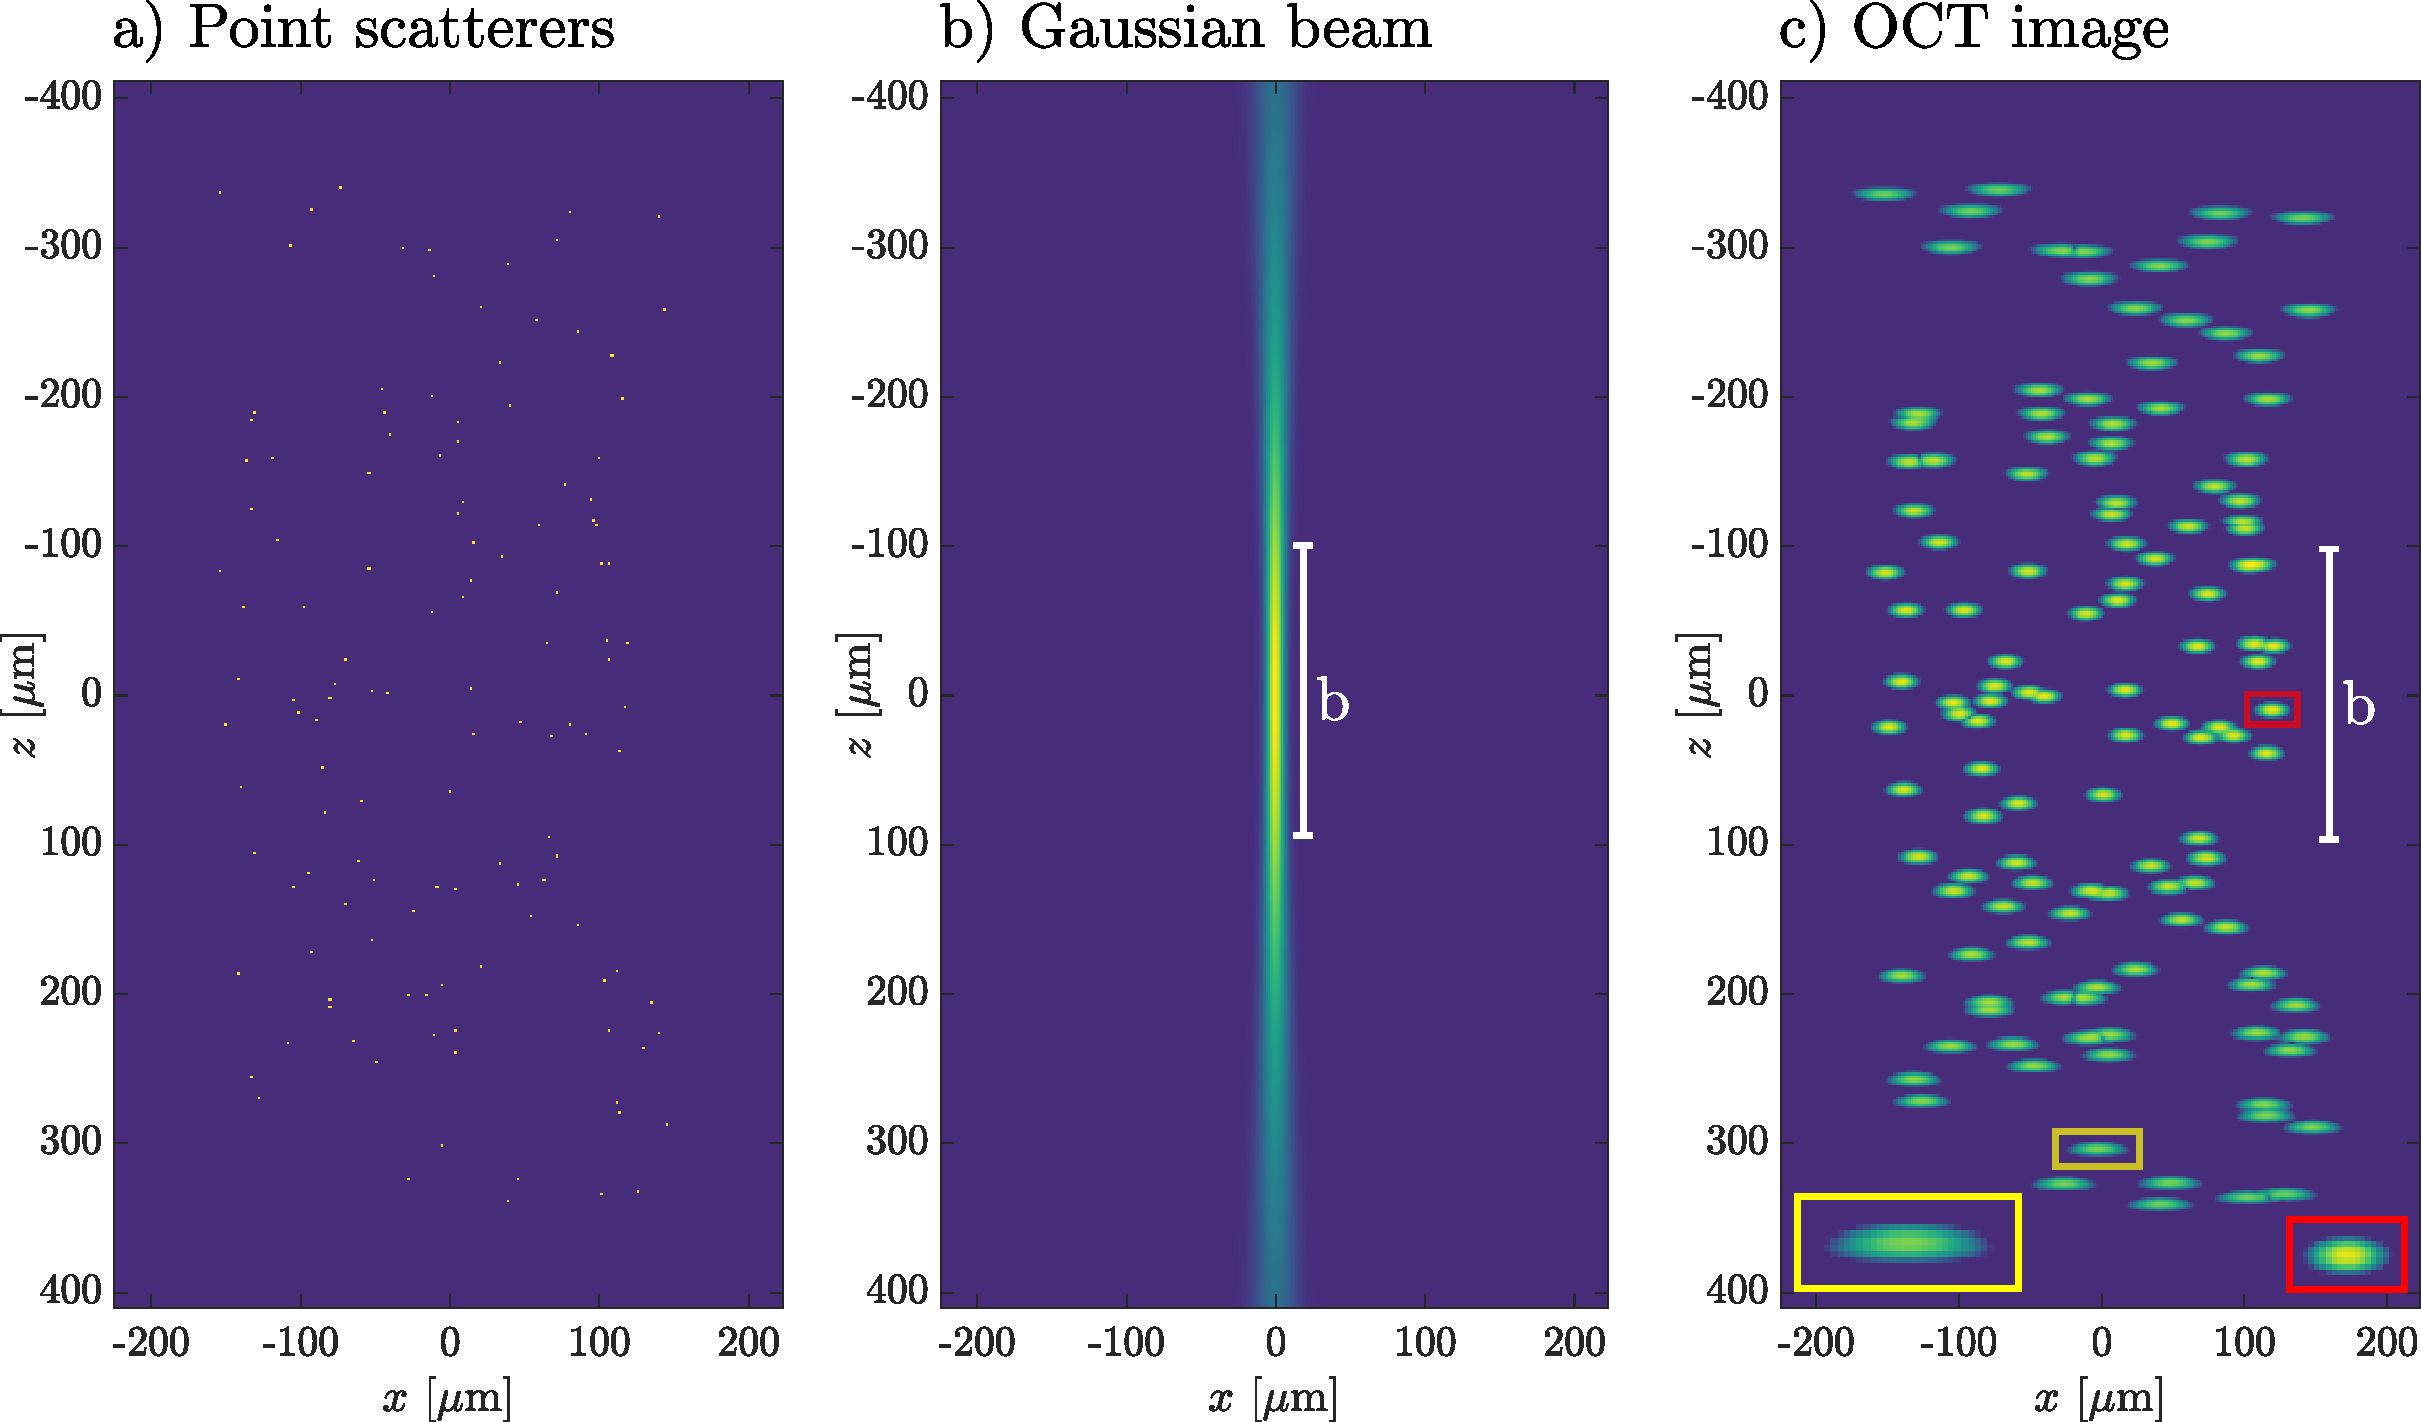
\includegraphics[width=\textwidth]{Figures/TheoreticalBasis/FM2.pdf}
    \caption{Simulation of an OCT image in low-NA regime. a) Sample consisting of randomly located point scatterers, b) Gaussian beam of the system with NA=$0.1$ and c) OCT image simulated using the forward model, displayed in logarithmic scale.}
    \label{fig:FM2}
\end{figure}

\iffalse Eq.~\ref{eq:conv} can be simplified in Fourier domain by invoking the convolution theorem and denoting the 2D Fourier transform over coordinates $(u, v)$ as $\text{FT}_{u,v}\{\cdot\}$,
\begin{equation}\label{eq:convFT}
    \hat{S}(q_x, q_y; k) = \int \hat{h}(q_x, q_y, z'; k) \hat{\eta}(q_x, q_y, z') dz'
\end{equation}
where $\hat{S} = \text{FT}_{x,y}\{S\}$, $\hat{h} = \text{FT}_{x,y}\{h\}$, $\hat{\eta} = \text{FT}_{x,y}\{\eta\}$, and $(q_x,q_y)$ are spatial frequency coordinates.

The PSF can be expressed as the product of the incident and detection complex probe beams, and given that OCT is based on a reflection (double-pass) geometry, the incident and collection beams are identical to $\sqrt{\mu_r}k|A(k)|g(x,y,z;k)$, where $\mu_r$ is the beam splitting power ratio, $|A(k)|^2$ is the power spectral density, and $g(x,y,z; k)$ is the focused beam produced by an input collimated beam at the back focal length of the optical system, thereby
\begin{equation}\label{eq:PSF1}
    h(x,y,z; k) = \mu_rk^2|A(k)|^2g^2(-x, -y, z; k),
\end{equation}
where the inversion of lateral coordinates $(x,y)$ is due to the reflection geometry. 

A plane wave decomposition of the focused probe beam yields~\ref{}
\begin{equation}~\label{eq:planewavedecomp}
    g(x,y,z ;k) = \frac{-i}{2\pi}\iint \frac{G(q_x, q_y, k)}{k_z}e^{i(q_xx+q_yy+k_zz)} dq_xdq_y,
\end{equation}
in terms of the generalized pupil function of the optical system $G(q_x, q_y, k)$, the object spatial frequencies $(q_x, q_y)$ and with $k_z(q_x, q_y) = \sqrt{k^2 - q_x^2 - q_y^2}$ that results from considering the optical wave vector $\mathbf{k}=(q_x, q_y, k_z)$.

The 2D Fourier transform over coordinates $(q_x, q_y)$ of Eq.~\ref{eq:planewavedecomp}, $\hat{g} =  \text{FT}_{x,y}\{g\}$, results in
\begin{equation}\label{eq:gFT}
    \hat{g}(q_x, q_y, z; k) = -i2\pi\frac{G(q_x, q_y; k)}{k_z(q_x, q_y)}e^{izk_z(q_x, q_y)}
\end{equation}

Now, computing the 2D Fourier transform over coordinates $(q_x, q_y)$ of Eq.~\ref{eq:PSF1} and using the convolution theorem, note that the transverse transfer function $\hat{h} \propto \hat{g} \otimes\hat{g}$ and it can be expressed using Eq.~\ref{eq:gFT} as
\begin{align}\label{eq:hFT}
    \hat{h}(-q_x, -q_y, z; k) = -4\pi^2\mu_rk^2|A(k)|^2  &\iint \frac{G(q_x', q_y'; k)}{k_z(q_x', q_y')} \frac{G(q_x-q_x', q_y-q_y'; k)}{kz(q_x-q_x', q_y-q_y')}... \nonumber\\
    &\times e^{-izk_z(q_x', q_y')}e^{-izk_z(q_x-q_x', q_y-q_y')}dq_x'dq_y'
\end{align}

To solve the integral in Eq.~\ref{eq:eq:hFT} it is possible to consider two complementary situations; near- and far-from-focus regimes. Recalling that $z=0$ at the focal plane, the far-from-focus regime is valid outside the DoF where effect of defocus is significant, where $z$ becomes large hence the phase term $|zk_z(q_x',q_y')|$ causes a rapid oscillation of the exponential term. This consideration allows to make use of the method of stationary phase~\ref{} which applies for integrals containing a rapidly oscillating complex exponential, such that the solution of the integral is found by evaluating the integral in the stationary point~\ref{}, that is, the point at which the argument of the complex exponential has zero gradient. The approximation of integral in Eq.\ref{eq:hFT} using the stationary point $(q_x', q_y') = (q_x/2, q_y/2)$ is
\begin{equation}\label{eq:hFT_fff}
    \hat{h}(-q_x, -q_y, z; k) \approx \frac{i4\pi}{-z}\mu_rk|A(k)|^2G^2\left(\frac{q_x}{2}, \frac{q_y}{2}; k\right)e^{-i2zk_z(\frac{q_x}{2}, \frac{q_y}{2})}.
\end{equation}

This expression shows explicit the amplitude and phase of the transverse transfer function of the system. The factor of $i=e^{i\frac{\pi}{2}}$ is equivalent to a phase of $\frac{\pi}{2}$ that is known as Gouy phase shift and it is characteristic of focused Gaussian beams~\ref{}. Decaying factor $1/z$ represents the signal decay with distance from focal plane that explains the loss of signal strength outside the DoF. In addition to the previous term, the other phase-dependent term is the phase factor that is responsible for the degradation of transverse resolution with increasing distance to the focal plane.

For the near-focus regime, consideration to apply the method of stationary phase to solve the integral in Eq,~\ref{eq:hFT} is not longer valid. In this case, $z$ is small hence the phase term $|zk_z(q_x',q_y')|$ oscillates slowly and the term $G(q_x', q_y'; k)$ can be considered narrowly peaked compared to the slow oscillation of the exponential term, and this can be used to derive an approximation solution~\ref{}, however, the derivation is rather extensive as explained in detail in Ref.~\ref{} and superfluous in this context considering that inside the DoF defocus correction is unnecessary when compared to the far-from-focus regime.

To finally derive the forward model for the far-from-focus regime, the transfer function of the system in Eq.~\ref{eq:hFT_fff} is replaced in Eq.~\ref{eq:convFT} to obtain
\begin{equation}\label{eq:SFT}
    \hat{S}_F(q_x, q_y; k) =  H_F(q_x, q_y; k)\int \frac{\tilde{\eta}(q_x, q_y, z')}{-z'}e^{-i2z'k_z(\frac{q_x}{2}, \frac{q_y}{2})} dz'.
\end{equation}
where $H_F(q_x, q_y; k) = i4\pi\mu_r k |A(k)|^2 G^2(-\frac{q_x}{2}, -\frac{q_y}{2}; k)$ is the depth-independent component of $\hat{h}$. Eq.~\ref{eq:SFT} is in the form of a Fourier transform with conjugate coordinates $z'$ and $2k_z(\frac{q_x}{2}, \frac{q_y}{2})$ and filtered by $H_F$. In fact, it has been proven that the forward model for the near-focus regime follow the same form that the forward model for far-from-focus, except that the Gouy phase shift and the decaying term $-1/z$ are not present and the depth-independent component of $\hat{h}$, denoted by $H_N(q_x, q_y; k)$, follows a slightly different functional form as can be seen in Ref.~\ref{}. Therefore, an unified approximate forward model for near- and far-from-focus regimes can be expressed in frequency domain as
\begin{equation}\label{eq:FM}
    \hat{S}(q_x, q_y; k) = H(q_x, q_y; k)\doublehat{\eta_a}(q_x, q_y, q_z)
\end{equation}
where $\doublehat{\eta_a}(q_x, q_y, q_z) = \text{FT}_{x,y,z}\{\rho(z)\eta(x,y,z)\}$ is the 3D Fourier transform of the attenuated scattering potential with spatial frequency coordinates $(q_x, q_y, q_z)$ where $q_z = -2\sqrt{k^2 - \left(\dfrac{q_x}{2}\right)^2 - \left(\dfrac{q_y}{2}\right)^2}$, and with the unified functions $H$ and $\rho$ given by
\begin{equation}
H(q_x, q_y; k) = 
\begin{cases}
    H_N(q_x, q_y; k)~~~\text{for}~~~|z| \ll z_R, \\
    H_F(q_x, q_y; k)~~~\text{for}~~~|z| \gg z_R,
\end{cases}
\end{equation}
\begin{equation}\label{eq:rhoz}
\rho(z) = 
\begin{cases}
    ~1~~~~~\text{for}~~~|z| \ll z_R, \\
    -\dfrac{1}{z}~~~\text{for}~~~|z| \gg z_R.
\end{cases}
\end{equation}

The forward model in Eq.~\ref{eq:FM} is a one-to-one mapping of the frequency distribution of the measured signal $\hat{S}$ and the frequency distribution of the attenuated scattering potential $\doublehat{\eta}_a$, with an additional filtering $H$ and with a coordinates conversion from the sample coordinates $(q_x, q_y, q_z)$ to the signal coordinates $(q_x, q_y, k)$, and this is responsible for the sample scattering potential appearing defocused in the acquired signal. The coordinate conversion causes a signal warping as a consequence of the indirect measurement of the scattering potential using an optical beam with particular wavenumber $k$.

To illustrate this, consider two point reflectors, one in the focal plane of the light probe and the other far from the focal plane as depicted in  Figure~\ref{}. Scattering follows the scattering vector relationship $\mathbf{q} = \mathbf{k}_{out} - \mathbf{k}_{in}$ that is a consequence of the momentum conservation, where $\mathbf{q}$ is the three-dimensional spatial frequency vector of the sample that is being measured and $\mathbf{k}_{out}$, $\mathbf{k}_{in}$ are wave vectors of the scattered and incident light, respectively. Input and scattered wavenumbers are within an acceptance angular range determined by the numerical aperture, describing what is known in diffraction tomography as an \textit{Ewald sphere}~\ref{}.

For the point in the focal plane, the whole angular view is collected in a single scan, therefore resolution is diffraction-limited. Also, note that a large NA provides a wider angular scan thus more frequencies components $\mathbf{q}$ of the sample are probed increasing lateral resolution.

For a point far from the focal plane, the acceptance angle becomes narrow, hence the frequency content $\mathbf{q}$ of the sample that can be probed in a single scan is smaller and resolution is decreased. Nonetheless, scanning the beam along the transverse coordinates increases the effective acceptance angle and it is possible to collected the frequency content of the sample even far-from-focus but along the sequential lateral scans, not in a single scan as for a point in the focal plane. This fact is related to the signal warping causing blurring of far-from-focus structures. For far-from-focus regime, $\mathbf{k}_{out}\approx - \mathbf{k}_{in}$ thus the measured frequency is $\mathbf{q} \approx -2 \mathbf{k}_{in}$, and the square magnitude yields the relation $4k = q_x^2 + q_y^2 + q_z^2$, that is the same obtained in the coordinate mapping of the forward model in Eq.~\ref{eq:FM}.
\fi


\section{Refocusing and computational aberration correction techniques in OCT}\label{CAC}

In the FM of Eq.~\ref{eq:FM}, the OCT signal $S$ is given by the sample potential $\eta$ modified by the system funcion $f^2$. From this model, it is possible to computationally obtain an approximate scattering sample potential $\tilde{\eta}$ by correcting the undesired effects present in the acquired signal $S$, that so far is only defocus due to the beam propagation, but additional aberrations may also be considered with further extensions presented below. There are several computational aberration correction techniques, some are oriented to correct for defocus to provide focal resolution throughout all depths, and others are oriented to correct for other types of aberrations that depend on the specific imaging system or even on the sample itself, in addition to defocus, and they are explained in the following sections.

To retrieve an approximate scattering sample potential from the acquired signal it is necessary to invert the forward model, what is known as an inverse scattering problem. In simple words, the FM gives the backscattering signal produced for a given scattering potential, while the inverse model gives the scattering potential that produced a given backscattering signal, and the latter is the interest in CAC.

For the derivation of CAC techniques, it is convenient to introduce the forward model in Fourier domain. To do so, the convolution theorem can be used to rewrite Eq.\eqref{eq:conv} as
\begin{equation}\label{eq:convFT}
    \hat{S}(q_x, q_y; k) = \int \hat{h}(q_x, q_y, z'; k) \hat{\eta}(q_x. q_y, z') \text{d}z'
\end{equation}
where $\hat{S}(q_x, q_y; k)=\text{FT}_{x,y}\{S(x,y;k)\}$, $\hat{h}(q_x, q_y, z; k)=\text{FT}_{x,y}\{h(x,y,z;k)\}$ is the depth-dependent frequency response of the PSF, and $\hat{\eta}(q_x, q_y, z)=\text{FT}_{x,y}\{\eta(x,y,z)\}$. Using an asymptotic approximation for the far-from-focus and near-focus cases~\ref{}, Eq.~\eqref{eq:convFT} can be simplified to
\begin{equation}\label{eq:FMft}
    \hat{S}(q_x, q_y; k) = H(q_x, q_y; k) \int \hat{\eta}(q_x. q_y, z') e^{iz'\sqrt{4k^2-q^2}} \text{d}z'
\end{equation}
where $H(q_x, q_y; k)$ is the space-invariant axial and lateral frequency response of the PSF, that is directly related to the optical transfer function of the system. In Eq.\eqref{eq:convFT}, a Gaussian beam is not assumed, contrary to the derivation of the FM in Eq.~\eqref{eq:FM}, so that $H(q_x, q_y; k)$ is a general function that may describe any aberration and not only defocus. Computational aberration correction makes use of the FM in frequency domain to reconstruct an approximate sample scattering potential.

\subsection{Interferometric synthetic aperture microscopy}

Interferometric synthetic aperture microscopy (ISAM) is a solution to the inverse scattering problem in OCT, and actually it is very similar to procedures used in synthetic aperture radar (SAR) and from this similarly arises the name ISAM. Eq.~\eqref{eq:FMft} can be considered as a Fourier integral with conjugate coordinates $z'$ and $q_z=\sqrt{4k^2-q^2}$, thus it is possible to write
\begin{equation}\label{eq:preISAM}
    \hat{S}(q_x, q_y; k) = H(q_x, q_y; k) \doublehat{\eta}(q_x. q_y, q_z)
\end{equation}
where $\doublehat{\eta} = \text{FT}_{x,y,z}\{\eta(x,y,z)\}$ is the 3D Fourier transform of the sample scattering potential. Eq.~\ref{eq:preISAM} is a one-to-one mapping between $\hat{S}$ and $\doublehat{\eta}$, contrary to convolution equation that is an all-to-all mapping between $S$ and $\eta$. The principle of operation of ISAM is to re-sample the Fourier spectrum of the acquired signal $S(x, y; k)$ in order to revert the coordinate warping, thereby the approximate scattering sample potential $\tilde{\eta}(x,y,z)$ can be expressed as

\begin{equation}\label{eq:ISAM}
    \tilde{\eta}(x,y,z) = \frac{1}{\rho(z)} \text{FT}^{-1}_{q_x,q_y.q_z}\left\{\big[H^{-1}(q_x, q_y; k) \hat{S}(q_x, q_y; k)\big]\bigg|_{k = \frac{1}{2}\sqrt{q_x^2 + q_y^2 + q_z^ 2}}\right\}.
\end{equation}

where $\rho(z) = -1/z$ countervails signal loss when far from focus. Eq.~\ref{eq:ISAM} consist in several steps; 1) computing the Fourier transform of the acquired signal along transverse spatial coordinates, 2) re-maping coordinates from $k$ to $q_z$ using the relation $k = \frac{1}{2}\sqrt{q_x^2 + q_y^2 + q_z^2}$, known as the Stolt mapping~\ref{}, and then 3) computing the three-dimensional inverse Fourier transform $\text{FT}^{-1}\{\cdot\}$. For ISAM, an ideal Gaussian beam is generally assumed, so that $H^{-1}$ is a weighting factor that will not introduce significant image distortion, thus it is usually set to unity. Normalization using $1/\rho(z)$ is not appropriate in practical terms to compensate for signal loss away from focal plane, thus it is commonly omitted or replaced with other depth normalization function. ISAM reconstruction is illustrated in Figure~\ref{fig:IM1} for the high-NA case of the simulated data in Fig.~\ref{fig:FM1}. The ISAM reconstruction shown in Fig.~\ref{fig:IM1}c) exhibit diffraction-limited resolution throughout all depths, and the major drawback present is the signal reduction, noticeable in points far from focal plane appearing dimmer than those in the focal plane.

\begin{figure}[htb!]
    \centering
    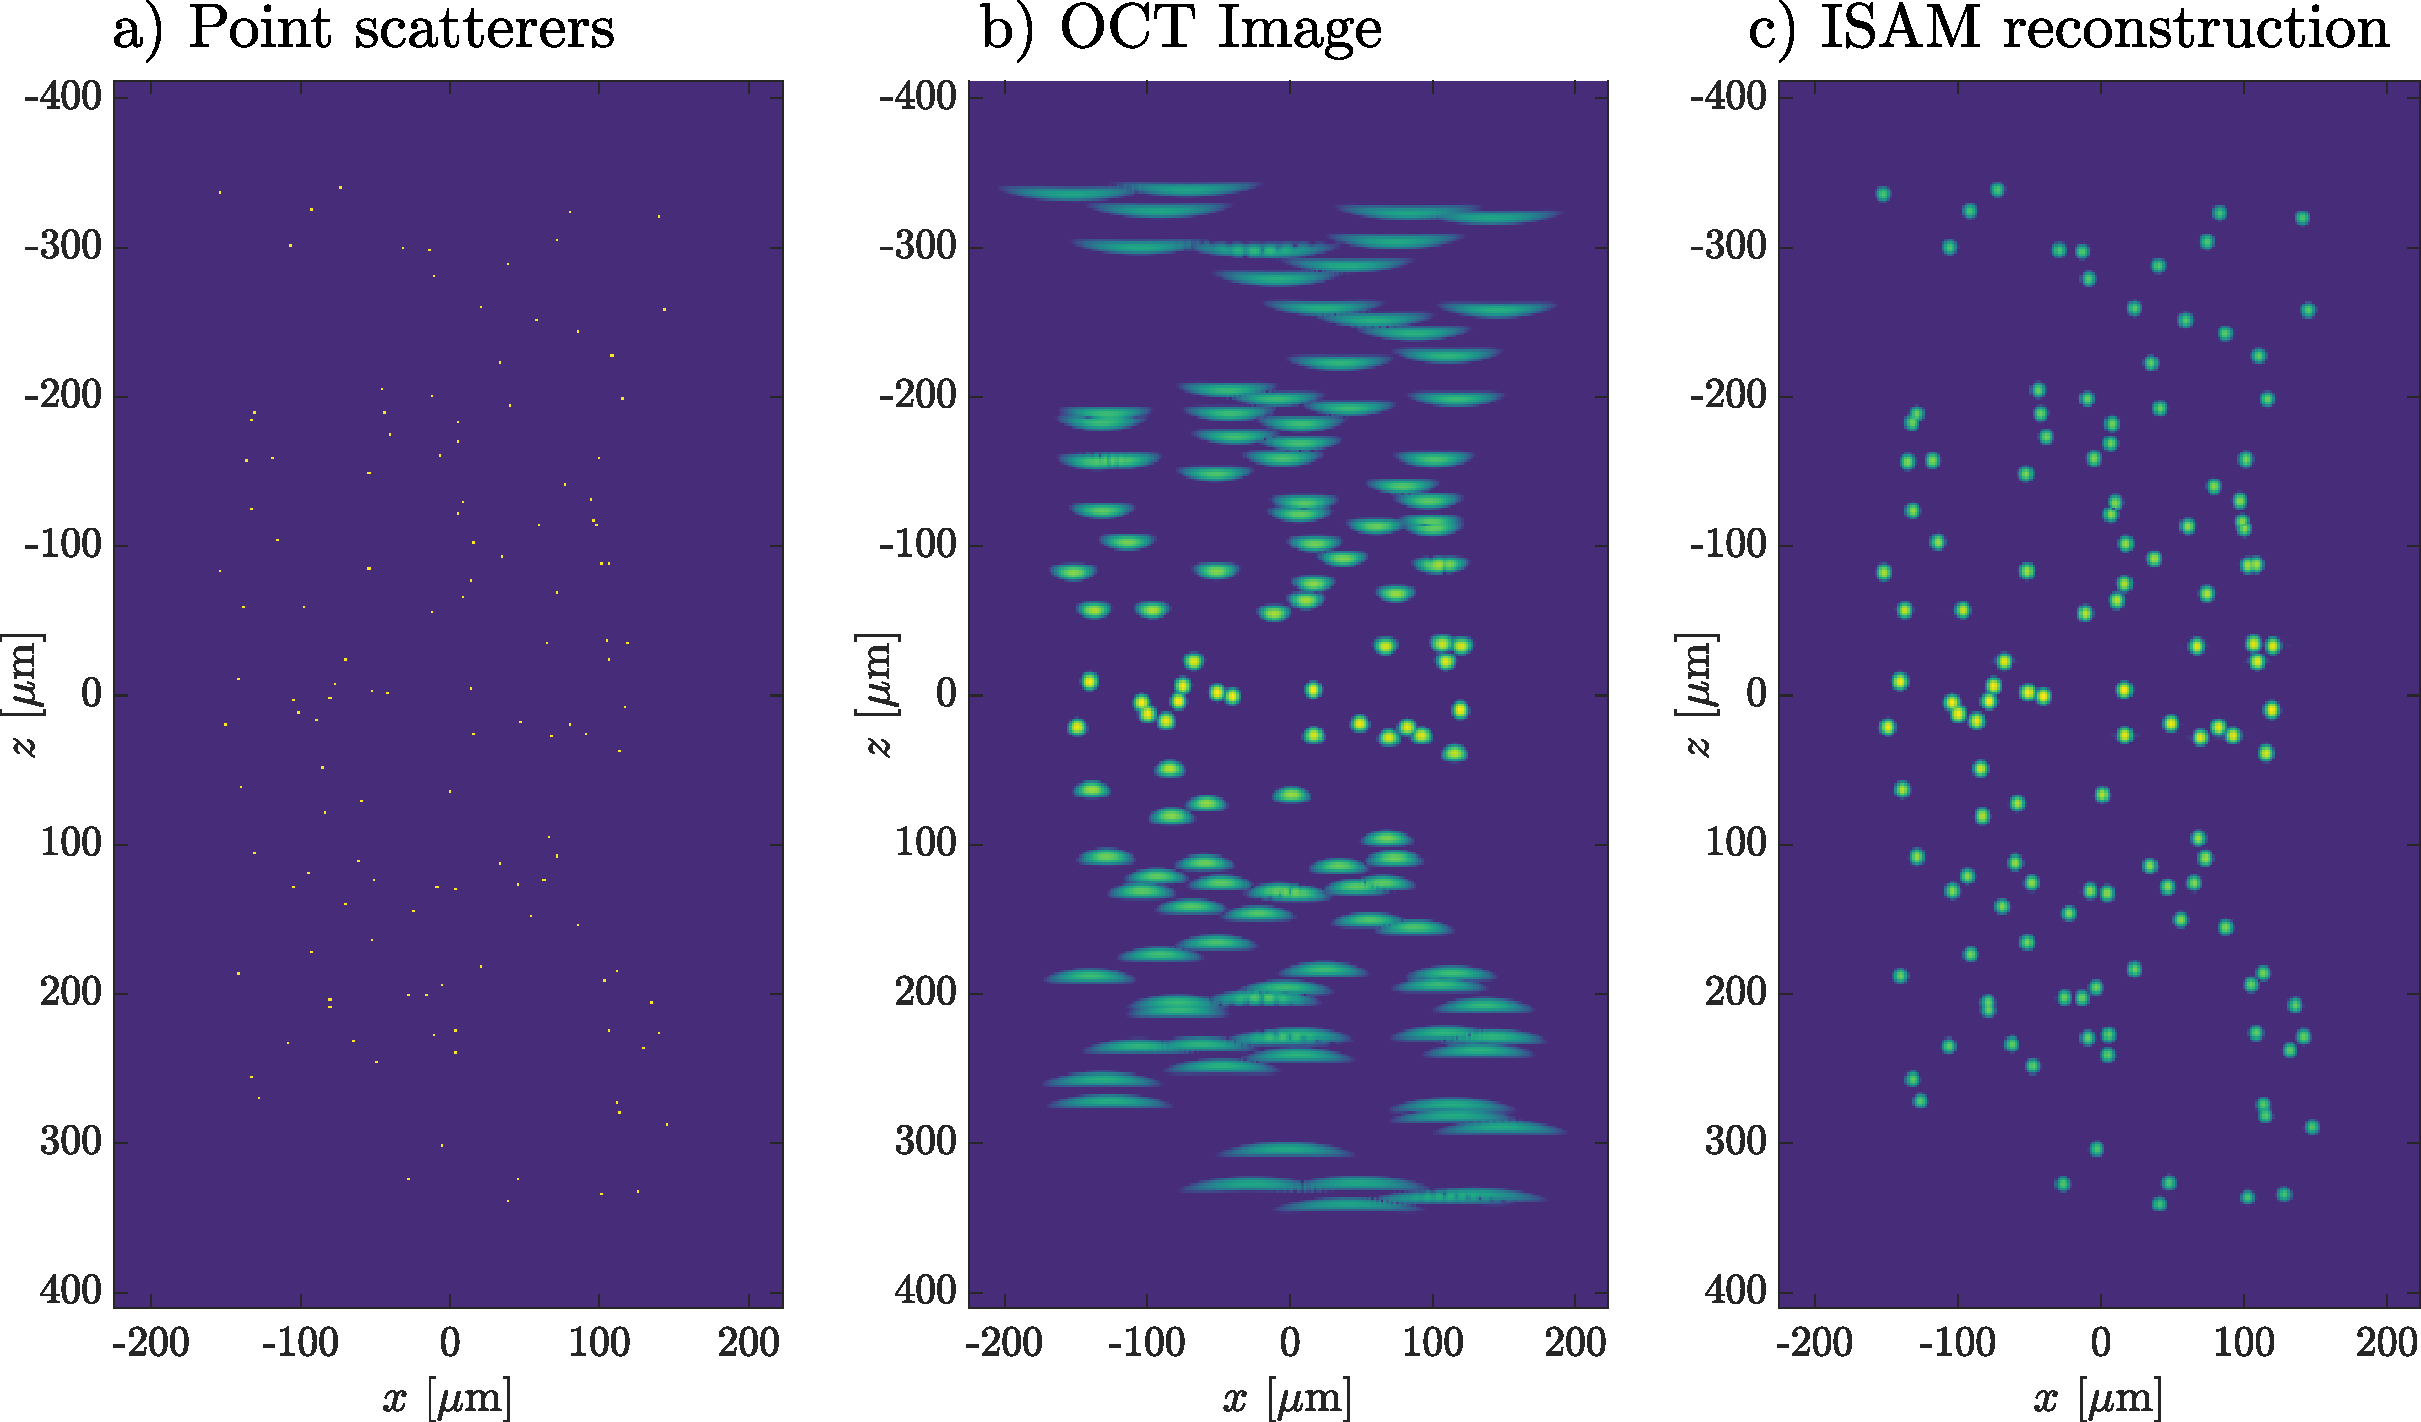
\includegraphics[width=\textwidth]{Figures/TheoreticalBasis/IM1.pdf}
    \caption{Illustration of ISAM operation. a) Sample consisting of randomly located point scatterers, b) OCT image simulated using the forward model c) ISAM reconstruction. b) and c) are displayed in logarithmic scale.}
    \label{fig:IM1}
\end{figure}
\iffalse
ISAM reconstruction is illustrated in Figure~\ref{fig:ISAM} for the case of the simulated data of sample with two point reflectors, one in the focal plane and the other above, outside the Rayleigh range. Note that point far-from-focus appears greatly blurred in Fig.~\ref{fig:ISAM}a), because the curvature distortion of the frequency components in the Fourier spectrum as seen in Fig.~\ref{fig:ISAM}b). ISAM resampling compensates the phase curvature as shown in Fig.~\ref{fig:ISAM}d), yielding an approximate sample scattering potential with diffraction-limited resolution throughout depth, although intensity of the point outside the Rayleigh range is lower than that of the point in the focal plane.

\begin{figure}[htb!]
    \centering
    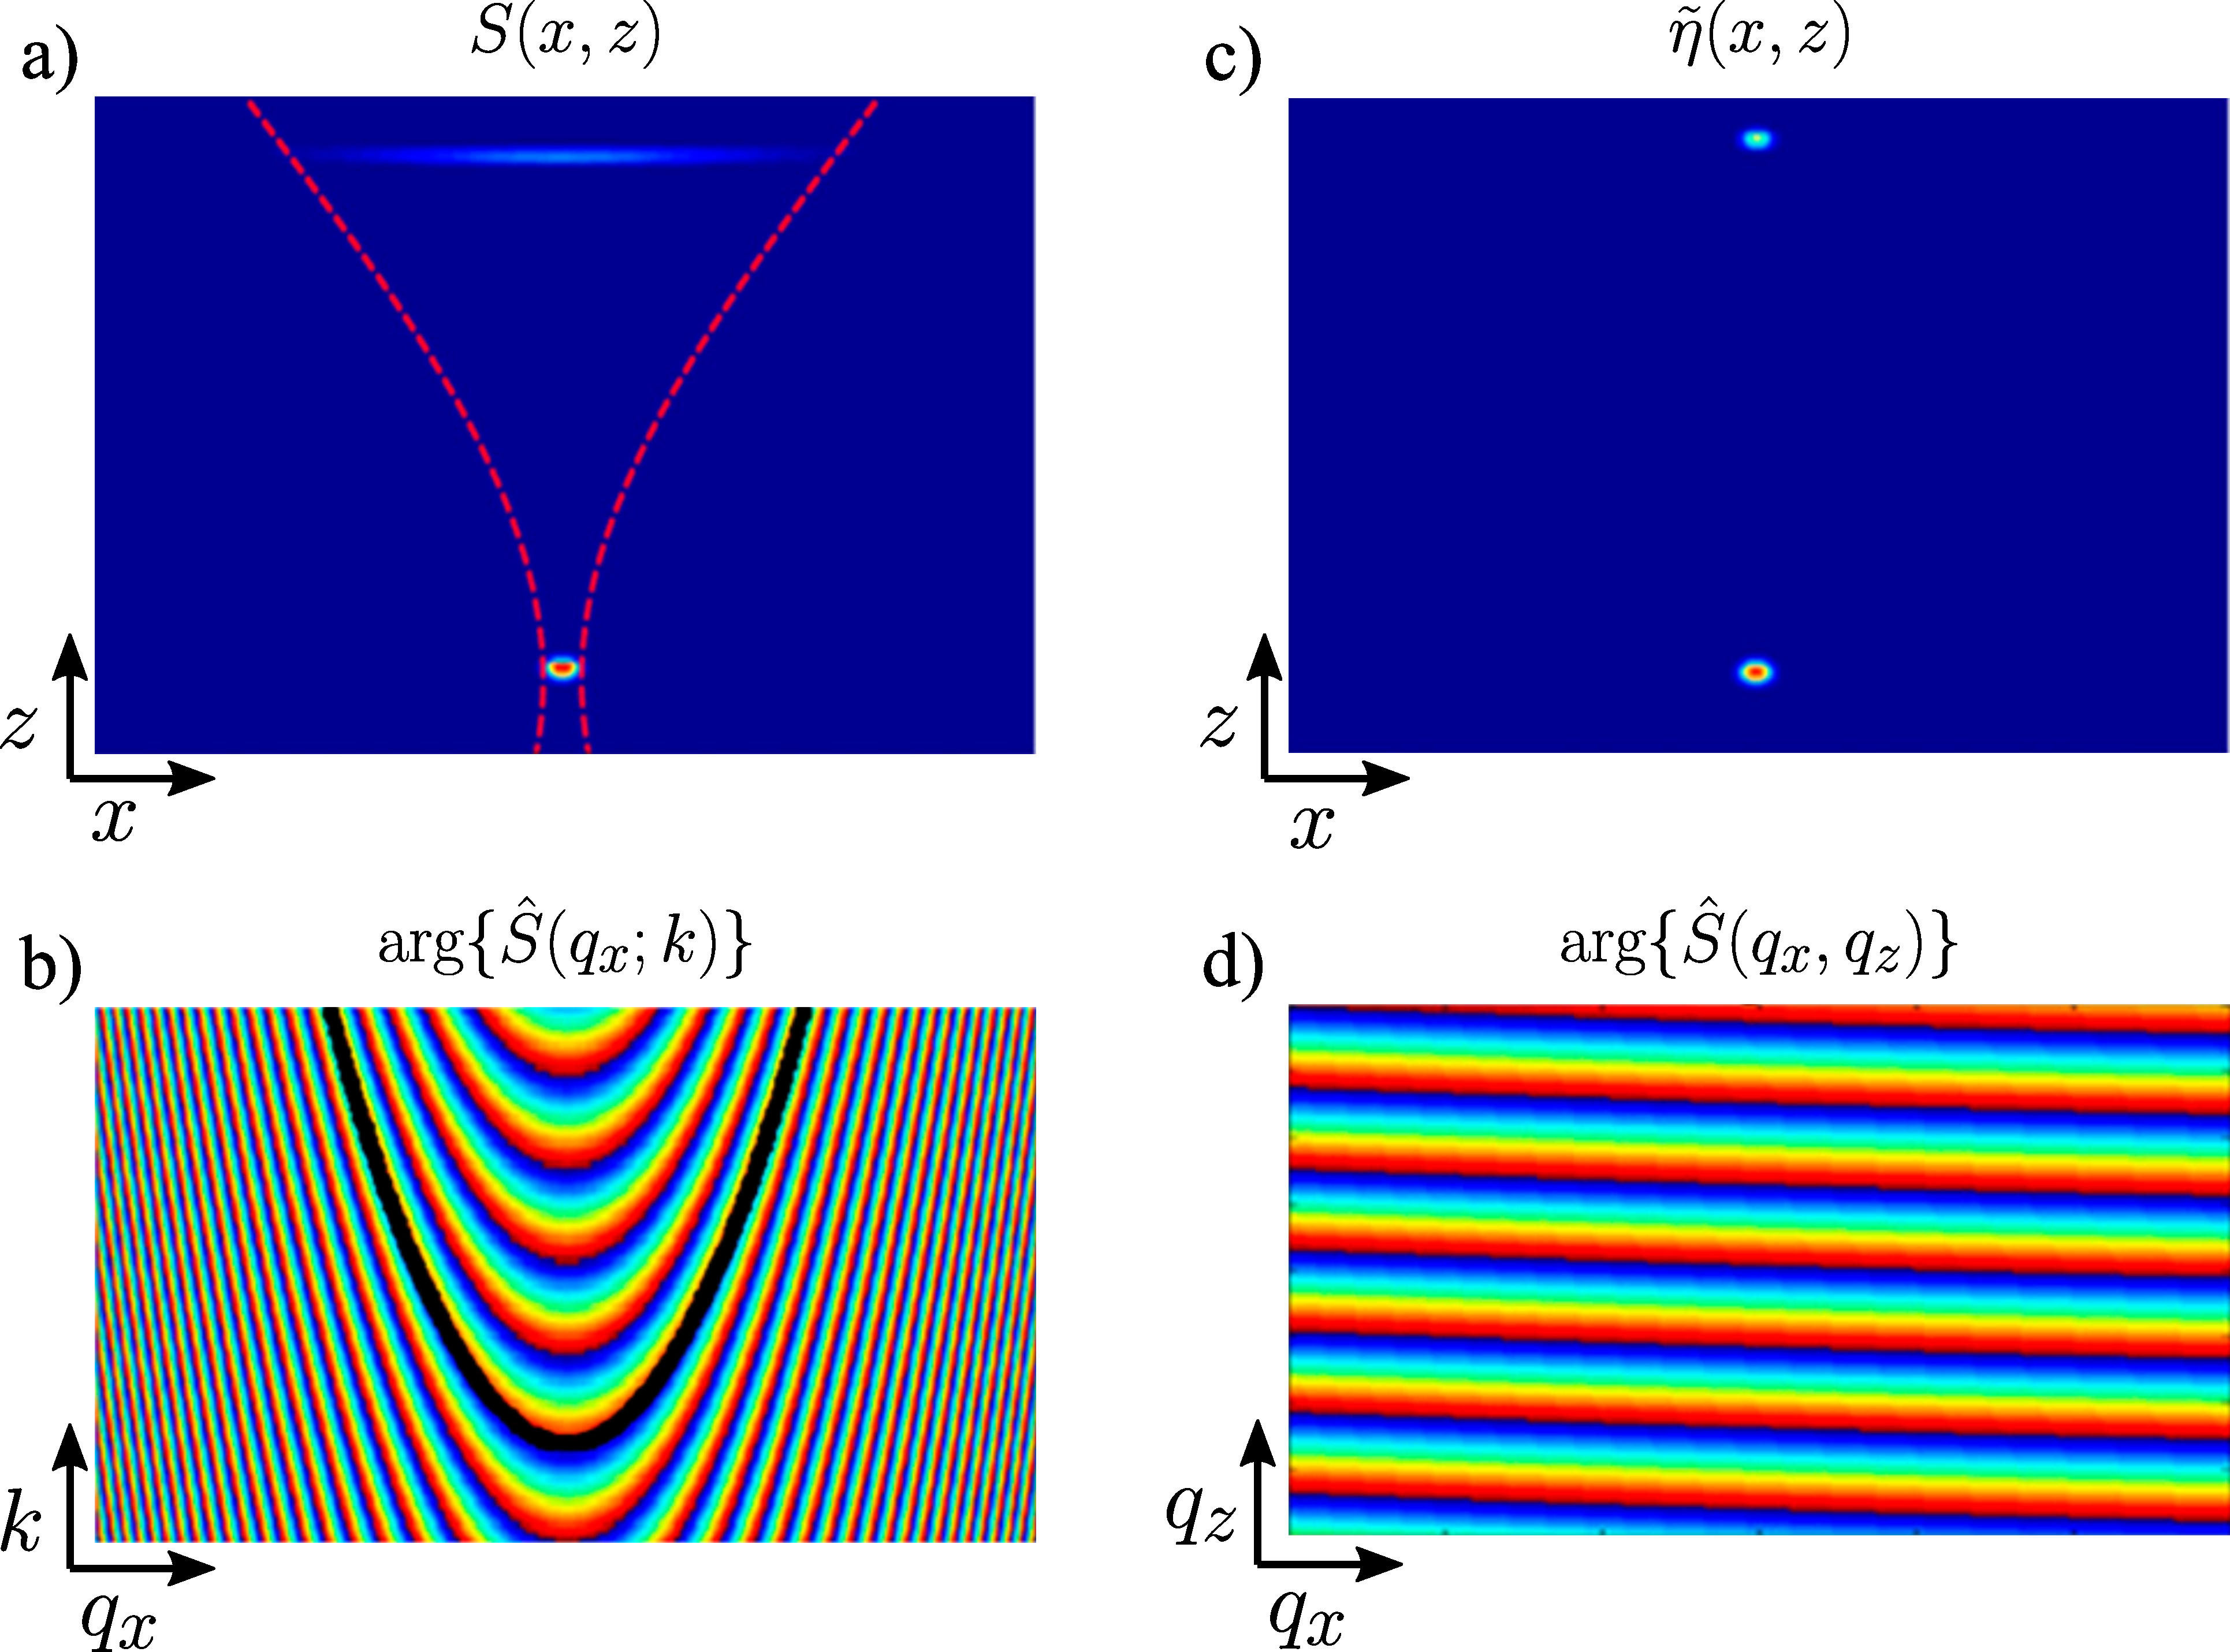
\includegraphics[width=.75\textwidth]{Figures/TheoreticalBasis/ISAM.pdf}
    \caption{Illustration of ISAM operation. a) Acquired B-scan image, b) phase map of its Fourier transform in $k$-space and d) in $q_z$-space after re-sampling, yielding ISAM reconstruction in c). Red line in a) represents the distribution of the focused beam when positioned in the central Aline, and black line in figure b) is an example of ISAM sampling curve. Figure adapted from Ref.~\ref{sudkamp}.}
    \label{fig:ISAM}
\end{figure}
\fi

ISAM, first proposed by Ralston et al.~\ref{}, has been used widely in the OCT community specially in high-resolution imaging where DoF is greatly reduced and computational correction of defocus is a key tool to extended the DoF~\ref{}, being the signal loss the major constrain. Extensions have been made to different imaging geometries and functional imaging, such as rotationally-scanned ISAM for endoscopic OCT~\ref{}, and polarization-sensitive ISAM~\ref{}. Furthermore, the development of ISAM have enable real-time in vivo visualization~\ref{}. 

\subsection{Digital refocusing}

ISAM reconstruction brings to focus all depths simultaneously, making use of the 3D frequency-content of the tomogram. In relatively low numerical aperture systems (NA $<$ 0.15) the re-sampling curve approximates a linear path which means that frequency content in not spread along depth, hence a 2D correction in the transverse plane determined for each plane $z$ independently is sufficient. To isolate a single plane $z_d$, inverse Fourier transform along $k$ of Eq.\eqref{eq:FMft} is computed and evaluated at $z=z_d$,
\begin{equation}\label{eq:preDefocus}
    \hat{S}(q_x,q_y; z_d) = \int H(q_x, q_y; k) \int \hat{\eta}(q_x,q_y, z_d) e^{iz\sqrt{4k^2-q^2}} e^{-i2z_dk} \text{d}z\text{d}k.
\end{equation}
Replacing $k=k_c + \Delta k$ with $\Delta k$ the difference between $k$ and central wavenumber $k_c$, the term $(\Delta k/k_c)^2$ is relatively small enough to be neglected, allowing to express $q_z=\sqrt{4k^2-q^2}$ under the paraxial approximation as
\begin{equation}\label{eq:qzAprox}
    q_z = 2k_c - \frac{q^2}{4k_c} + 2\Delta k.
\end{equation}

Replacing $q_z$ in Eq.\eqref{eq:preDefocus}, as well as using convolution theorem to rewrite Foruier integral along $k$, it is possible to obtain
\begin{align}\label{eq:preDefocus2}
    \hat{S}(q_x,q_y; z_d) &= \int H(q_x, q_y; k) \int \hat{\eta}(q_x,q_y, z_d) e^{iz(2k_c - q^2/4k_c + 2\Delta k)} e^{-i2z_d(k_c+\Delta k)} \text{d}z\text{d}\Delta k \nonumber \\
    &= \int H(q_x, q_y; k) \int \hat{\eta}(q_x,q_y, z_d) e^{i2(z-z_d)k_c} e^{-izq^2/4k_c} e^{i2(z-z_d)\Delta k} \text{d}z\text{d}\Delta k \nonumber \\
    &= H(q_x, q_y; z_d) \otimes \left[ \int \hat{\eta}(q_x,q_y, z_d) e^{i2(z-z_d)k_c} e^{-izq^2/4k_c}  \delta(2z-2z_d) \text{d}z\right] \nonumber \\
    &= H(q_x, q_y; z_d) \otimes \left[ \hat{\eta}(q_x,q_y, z_d) e^{-iz_dq^2/4k_c}  \right]
\end{align}
where the convolution is performed along axial axis. The depth-dependent part of $Hq_x,q_y;z_d)$ is related to the axial PSF that can be approximated to a delta function, so that $H(q_x, q_y; z) \propto H(q_x, q_y)\delta(z-z_d)$, which can be replaced in Eq.~\eqref{eq:preDefocus2} to obtain its inverse Fourier transform along $\mathbf{q}$ as
\begin{equation}\label{eq:defocusFT}
    S(x, y; z_d) = \text{FT}^{-1}_{q_x, q_y}\left\{H(q_x, q_y)\hat{\eta}(q_x, q_y; z_d) e^{-iz_dq^2/4k_c}\right\},
\end{equation}

Eq.~\eqref{eq:defocusFT} is an expression with a form widely known in digital refocusing methods based on scalar diffraction models such as the Fresnel propagator~\cite{}, where the exponential term is a quadratic phase term responsible of depth-varying defocus. A straightforward inversion of Eq.~\eqref{eq:defocusFT} provides an approximate refocused sample scattering potential by
\begin{equation}\label{eq:refocus}
    \tilde{\eta}(x,y; z_d) = \text{FT}^{-1}_{q_x, q_y}\left\{H(q_x, q_y)\hat{S}(q_x, q_y; z_d) e^{iz_dq^2/4k_c}\right\},
\end{equation}
Similarly to ISAM, an ideal Gaussian beam can be assumed and $H$ is set to unity.
Although reconstruction using digital refocusing of Eq.\eqref{eq:refocus} is not complex, there are conceptual differences with ISAM reconstruction. In digital refocusing, each depth is brought to focus independently, applying an appropriate quadratic phase term, whereas ISAM reconstruction restores the entire volume simultaneously re-sampling the signal in Fourier domain. More importantly, due to the paraxial approximation in Eq.\eqref{eq:qzAprox}, digital refocusing methods are valid only for low-NA regimes, where there is not coordinates warping that mixes lateral and axial information. Digital refocusing is illustrated in Figure~\ref{fig:IM2} for the low-NA case of the simulated data in Fig.\ref{fig:FM2}, and note that digital refocused image of Fig.~\ref{fig:IM2}c) exhibit diffraction-limited resolution throughout all depth.

\begin{figure}[htb!]
    \centering
    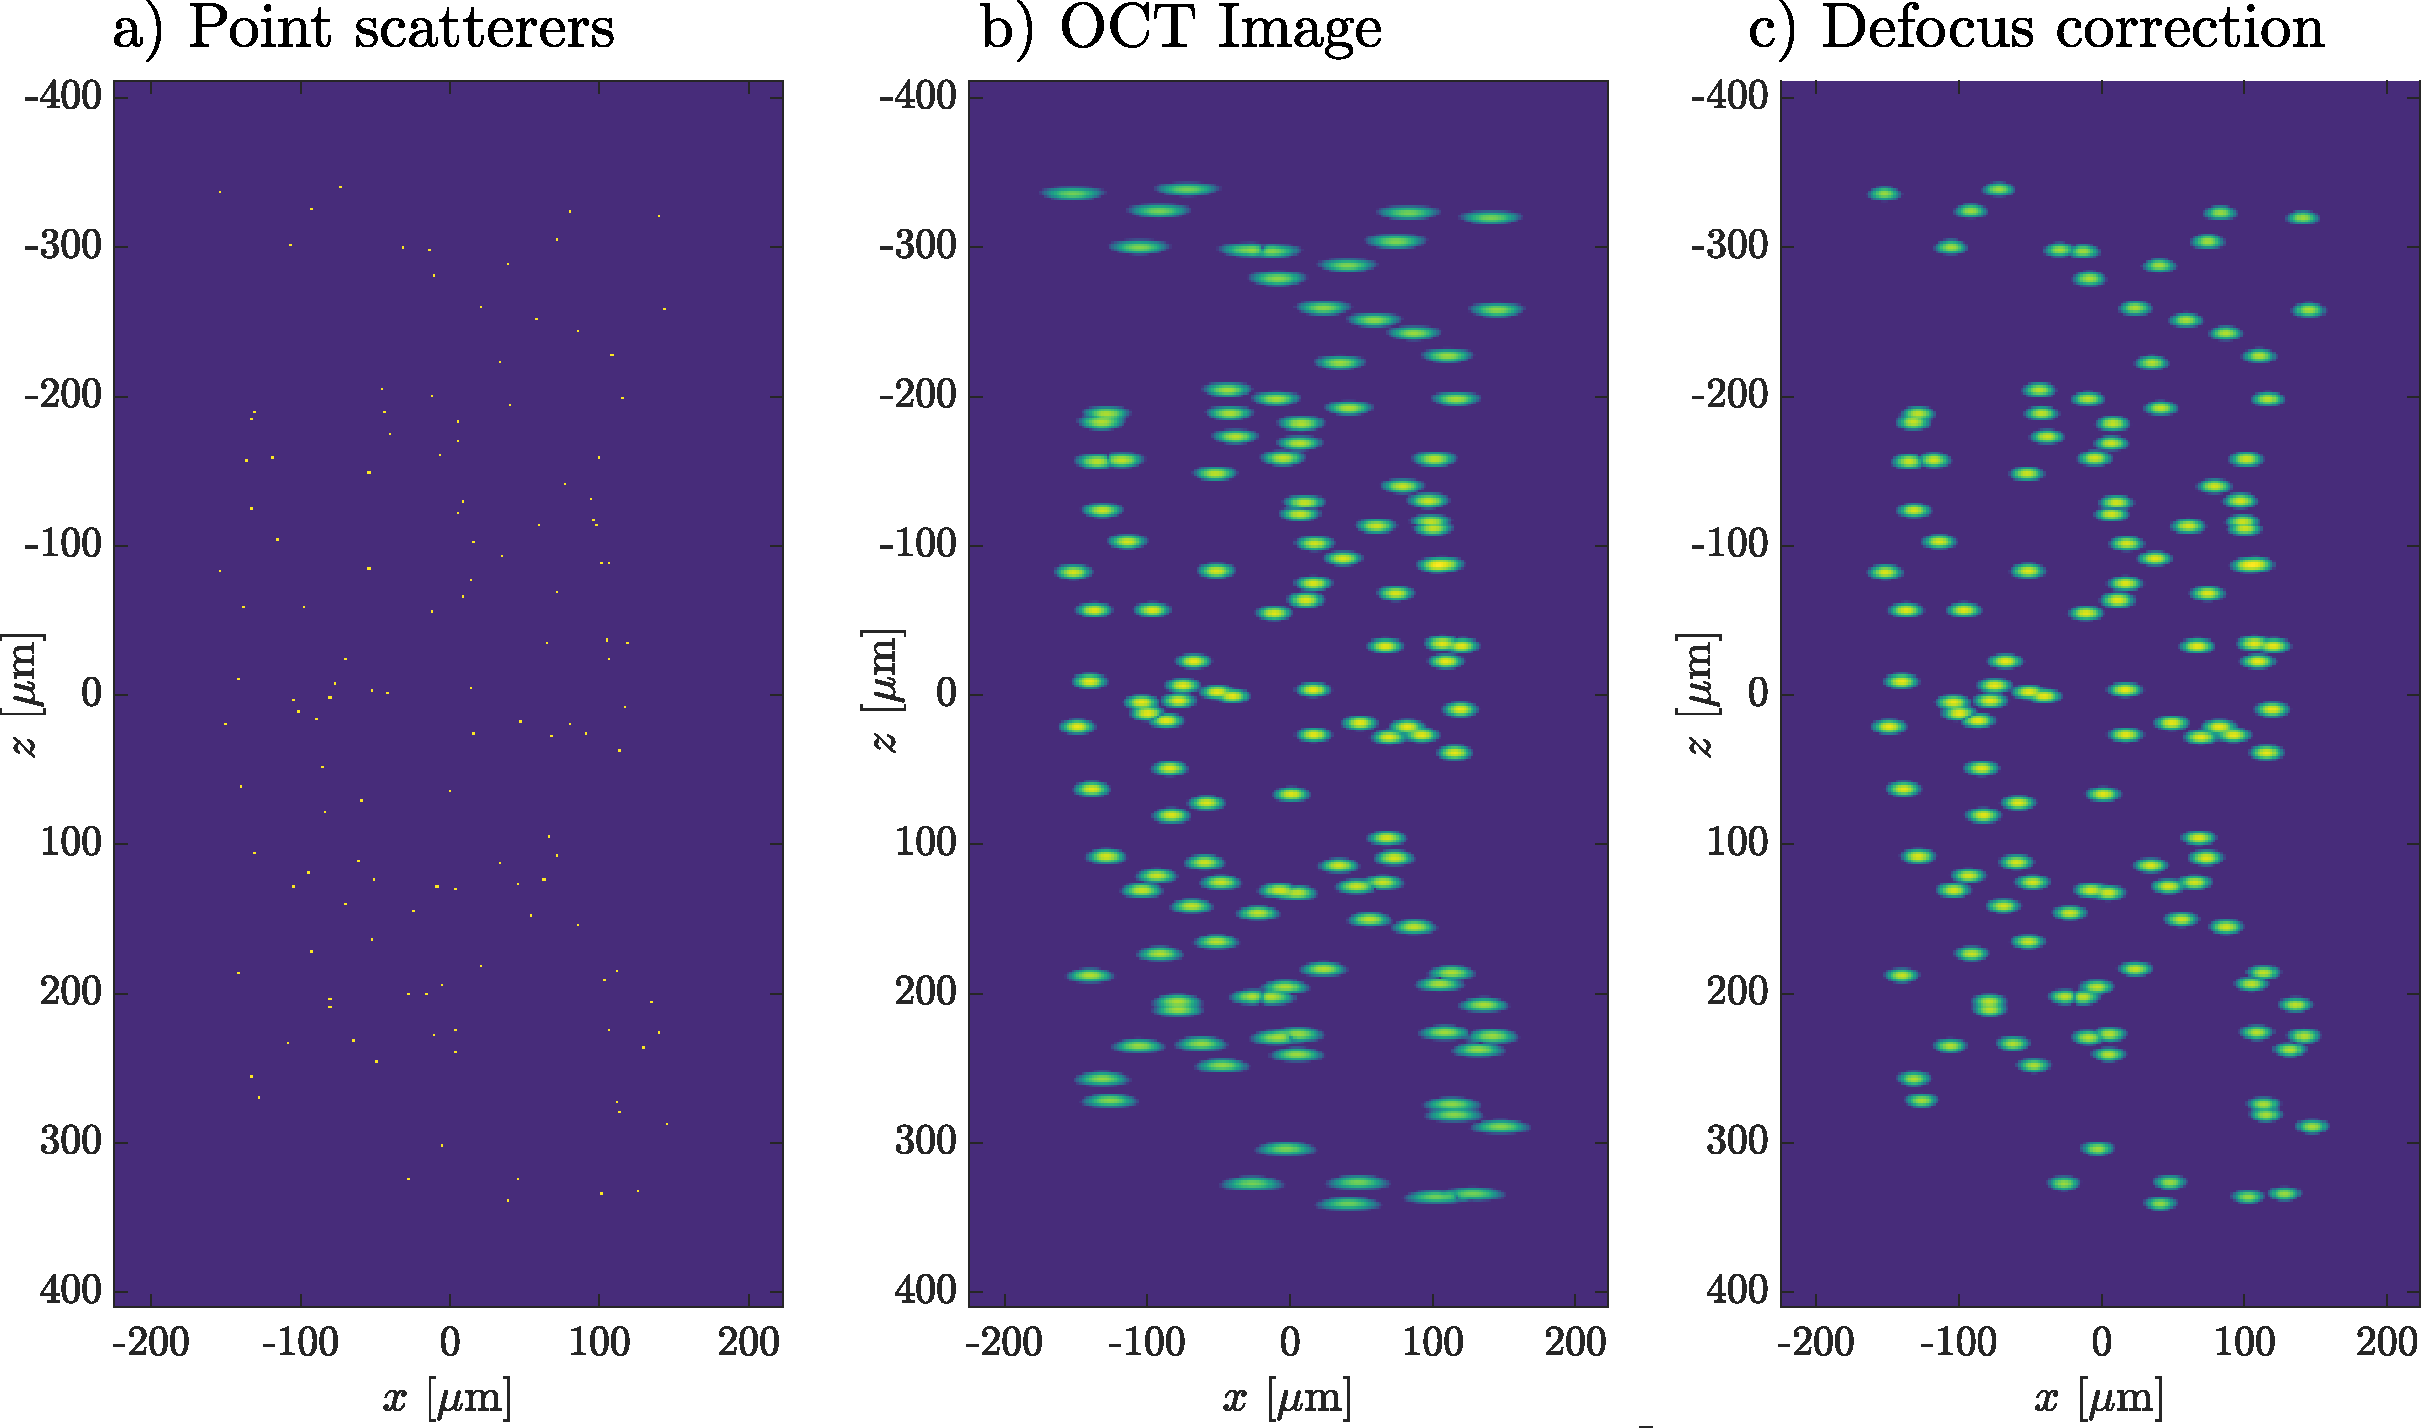
\includegraphics[width=\textwidth]{Figures/TheoreticalBasis/IM2.pdf}
    \caption{Illustration of digital refocusing. a) Sample consisting of randomly located point scatterers, b) OCT image simulated using the forward model c) Digital refocused. b) and c) are displayed in logarithmic scale.}
    \label{fig:IM2}
\end{figure}

\subsection{Computational adaptive optics}

Aberrations are wavefront distortions with respect to a reference wavefront, affecting image quality in several imaging techniques such as OCT. Several applications in OCT have benefited from aberration correction, whether using specific optical systems, hardware-based adaptive optics or computational adaptive optics. For instance, in retinal imaging, the probe beam is focused onto the retina using the optical system of the eye itself (cornea/lens) that may produce an distorted wavefront affecting image quality. In particular, the wavefront in high NA systems is more susceptible to be distorted by imperfections of the optical systems or even the sample itself.

Defocus introduced in the propagation of light is intrinsic to the Gaussian probe beam, for this reason, it is not considered as an optical aberration, which in this case are wavefront deviations from the ideal wavefront of a Gaussian beam. This can be noted in Eq.\eqref{eq:FMft}, where defocus arises from the exponential term whereas wavefront distortions can be modelled by $H(q_x, q_y; k)$ that is related to the effective generalized pupil of the optical system, resulting from the convolution of the illumination and detection generalized pupils, that are identical in OCT given the double-pass geometry.

Recalling the forward model in frequency domain, it is possible to invert Eq.\eqref{eq:preISAM} to obtain an aberration-corrected OCT signal as
\begin{equation}\label{eq:preCAO}
    \tildehat{S}(q_x, q_y; k) = H^{-1}(q_x, q_y; k) \hat{S}(q_x, q_y; k).
\end{equation}
where, $H^{-1}(q_x, q_y; k)$ acts as a frequency filter, which depends on spatial frequency and spectral domains, therefore it can address chromatic aberrations~\cite{}. Given the relatively narrow spectrum of the light sources used in OCT, in practical scenarios it is convenient to assume a $k$-independent filter $H(q_x,q_y)$, which is the same for all depths. In HAO, the correction filter $H(q_x,q_y)$ is applied directly in situ to compensate for the distortions of the Gaussian beam, but, because coordinate re-sampling is not included in this expression, $\tilde{S}(q_x, q_y; k)$ is an aberration-corrected signal rather than the sample scattering potential, it means that defocus will be present yet in the acquired images. To correct for defocus using HAO, a depth-dependent phase filter is necessary but it is not possible with current hardware such as deformable mirrors. In the case of CAO, the filter is applied in post-processing. ISAM or digital refocusing can be combined with aberration correction to obtain aberration-free images with focal resolution throughout all depths, namelely $\tilde{\eta}(x, y, z)$. For ISAM reconstruction, note that $\tildehat{S}(q_x, q_y; k)$ is explicit in Eq.\eqref{eq:ISAM}. For low-NA regime, the depth-invariant filter $H(q_x,q_y; z_d)$ can be generalized in Eq.\eqref{eq:refocus} to a depth-dependent filter $H(q_x,q_y)$ that includes the exponential term, resulting in 
\begin{equation}\label{eq:CAC}
    \tilde{\eta}(x, y; z_d) = \text{FT}_{q_x,q_y}^{-1}\left\{H^{-1}(q_x, q_y; z_d) \hat{S}(q_x, q_y; z_d)\right\}.
\end{equation}

In this case, defocus in treated as an aberration contained in the correction filter $H^{-1}(q_x, q_y; z_d)$. The procedure to obtain an aberration-correction sample scattering potential using Eq,\eqref{eq:CAC} is rather simple, note that it is a deconvolution in Fourier domain. The key point in computational adaptive optics is to determine the appropriate correction filter. Determination of $H^{-1}$ 

\subsection{Phase stability requirement} \label{sec:phaseStab}